\input{preamble}
\input{format}
\input{commands}

\begin{document}

\begin{Large}
    \textsf{\textbf{Homework 9}}
    
    \textbf{DFT \& IDFT}
\end{Large}

\vspace{1ex}

\textsf{\textbf{Student:}} \text{Yuanyuan Zhao, 2300013077, School of EECS}, \href{mailto:your.email@hotmail.com}{\texttt{zhaoyuanyuan@stu.pku.edu.cn}}\\
\textsf{\textbf{Lecturer:}} \text{Yisong Chen}
% \href{mailto:your.email@hotmail.com}
% {\texttt{chenyisong@pku.edu.cn}}\\


\vspace{2ex}

\begin{problem}{DFT \& IDFT Algorithm Design}{algo}
    We implement our customized DFT and IDFT algorithm in myDFT2\_fast.mlx and myIDFT2\_fast.mlx, and the image-processing script is DFT\_IDFT.mlx.
\begin{enumerate}[(a)]
    \item \textbf{DFT \& IDFT Process}
    \begin{enumerate}[label = (\roman*)]
        \item Build the wave basis 
        $$\phi_{u,v}(x,y) = e^{-i2\pi (\frac{ux}{M}+\frac{vy}{N})}$$
        $$
        \sum_{x=0}^{M-1} \sum_{y=0}^{N-1}\phi_{u,v}(x,y)\phi^*_{u',v'}(x,y)=
        \begin{cases}
        MN &\text{if}\ u=u' \text{and}\ v=v'\\
        0&\text{otherwise}
        \end{cases}
        $$
        Because of the above equation, normalization is required in subsequent IDFT process.
        
        
        \item Calculate the coefficient 
        $$F(u,v) = \sum_{x=0}^{M-1} \sum_{y=0}^{N-1} f(x,y)\phi_{u,v}(x,y)$$
        For all the pixel $(x, y)$ in the image, accumulate their similarity with frequency $(u/M, v/N)$, that is, $f(x,y)\phi_{u,v}(x,y)$.

        \item Move low frequencies to the center for visualization
        \begin{verbatim}
                    F_shifted = fftshift(F); 
        \end{verbatim}

        \item Show the magnitude, phase, real part and imaginary part of $F$
        $$log_{mag}=\log(1 + \vert F_{shifted}\vert)$$
        \begin{verbatim}
                    magnitude = mat2gray(log_mag);
                    phase = angle(F);
                    real_part = real(F);
                    imag_part = imag(F);  
        \end{verbatim}

        \item Reconstruct the image
        $$f(x,y)=\frac{1}{MN}\sum_{u=0}^{M-1}\sum_{v=0}^{N-1}F(u,v)\phi^*(x,y)$$
        For all the frequencies $(u/M, v/N)$ as a wave basis, accumulate their contribution to the image, that is, $F(u,v)\phi^*(x,y)$. In the equation, $\frac{1}{MN}$ is the normalization coefficient calculated in (i) and $\phi^*$ is the complex conjugate of $\phi$.
    \end{enumerate}

    
    \item \textbf{Implementation 1: For-Loop Version}
    
        To calculate the coefficient $F$, we need to traverse all pairs of $(u,v)$ where $u=0,1,...,M-1, v=0,1,...,N-1$. And for each $(u,v)$, the coefficient is based on all the pixels $(x,y)$. So, the time complexity of the for-loop algorithm is $O(M^2N^2)$, which is inacceptably time consuming.
        Specific implementation can be found in myDFT.mlx and myIDFT.mlx.
    \item \textbf{Implementation 2: Matrix Multiplication Speedup}
    
        To speed up the process, we calculate the vertical and horizontal DFT and IDFT kernel in advance.
        Specific implementation can be found in myDFT2\_fast.mlx and myIDFT2\_fast.mlx.
        \begin{verbatim}
                    u = (0:M-1)';
                    x = 0:M-1;
                    Wx = exp(-1i * 2 * pi * (u * x) / M);

                    v = (0:N-1)';
                    y = 0:N-1;
                    Wy = exp(-1i * 2 * pi * (v * y) / N);

                    x = (0:M-1)';
                    u = 0:M-1;
                    iWx = exp(1i * 2 * pi * (x * u) / M); 
                    
                    y = (0:N-1)';
                    v = 0:N-1;
                    iWy = exp(1i * 2 * pi * (y * v) / N);  
        \end{verbatim}
        Then the Fourier Transform can be carried out with the weight matrix.
        $$F = Wx * f * Wy$$
        $$f = (iWx * F * iWy) / MN$$
  
    
\end{enumerate}
\end{problem}
\begin{problem}{Low \& High Frequency Filter}{filter}

\begin{enumerate}[(a)]
    \item \textbf{Build the Filter}
    
        Choose appropriate Cutoff Frequency $D_0$ and we have \begin{verbatim}
                    H_low = double(D <= D0);
                    H_high = double(D > D0);
        \end{verbatim}

    
    
    \item \textbf{Calculate the Filtered Coefficient}
        \begin{verbatim}
                    F_low = F_shifted .* H_low;
                    F_high = F_shifted .* H_high;
        \end{verbatim}
    \item \textbf{Reconstruct the Filtered Image}
        \begin{verbatim}
                    img_low = myIDFT2_fast(F_low);
                    img_high = myIDFT2_fast(F_high);
        \end{verbatim}
\end{enumerate}
\end{problem}

\begin{figure}[htbp]
    \centering 
    \begin{minipage}{0.8\textwidth} 
        \centering 
        
        \begin{subfigure}[b]{0.45\linewidth} 
            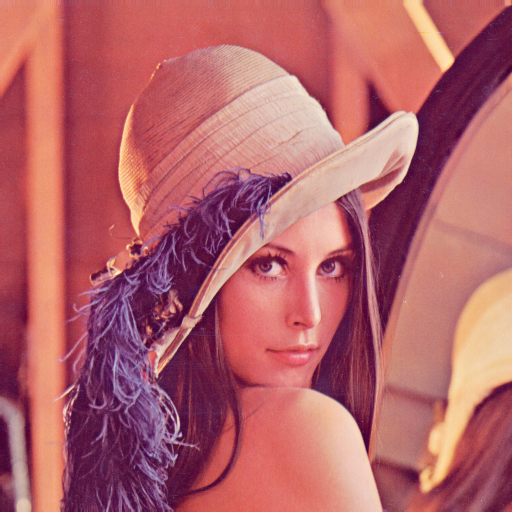
\includegraphics[width=\linewidth]{images/lena.png}
            \caption{Original Image}
        \end{subfigure}
        \hfill
        \begin{subfigure}[b]{0.45\linewidth}
            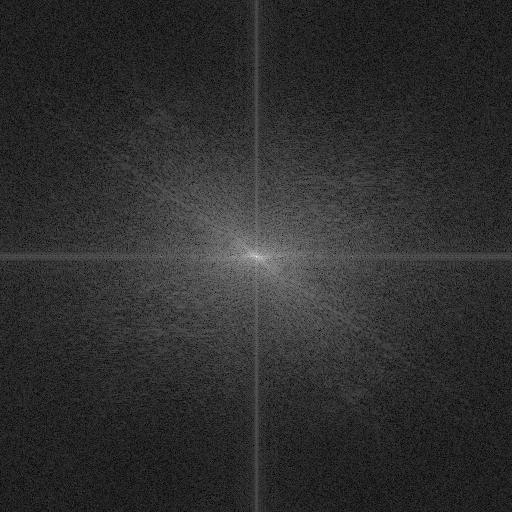
\includegraphics[width=\linewidth]{images/lena_R_magnitude.jpg}
            \caption{R-Magnitude}
        \end{subfigure}

        \vspace{0.5cm}
        \begin{subfigure}[b]{0.45\linewidth}
            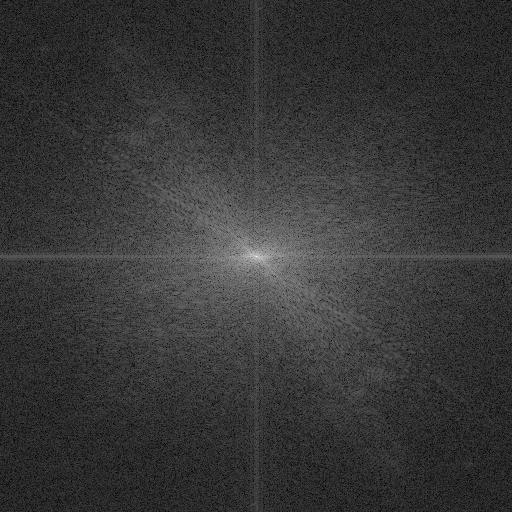
\includegraphics[width=\linewidth]{images/lena_G_magnitude.jpg}
            \caption{G-Magnitude}
        \end{subfigure}
        \hfill
        \begin{subfigure}[b]{0.45\linewidth}
            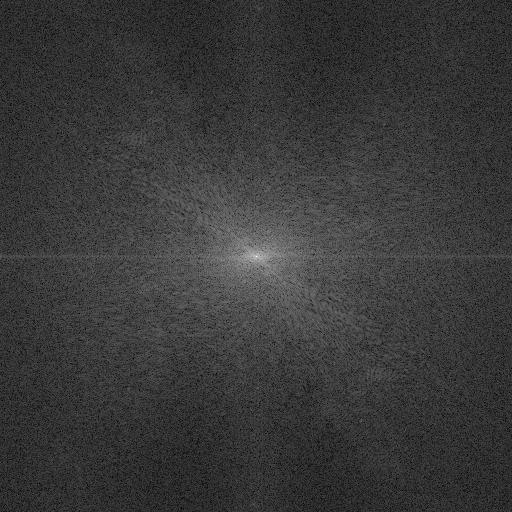
\includegraphics[width=\linewidth]{images/lena_B_magnitude.jpg}
            \caption{B-Magnitude}
        \end{subfigure}

        \caption{Lena: Magnitude in R, G, B channels}
        \label{fig:lena}
    \end{minipage}
\end{figure}

\begin{figure}[htbp]
    \centering 
    \begin{minipage}{0.8\textwidth} 
        \centering 
        
        \begin{subfigure}[b]{0.45\linewidth} 
            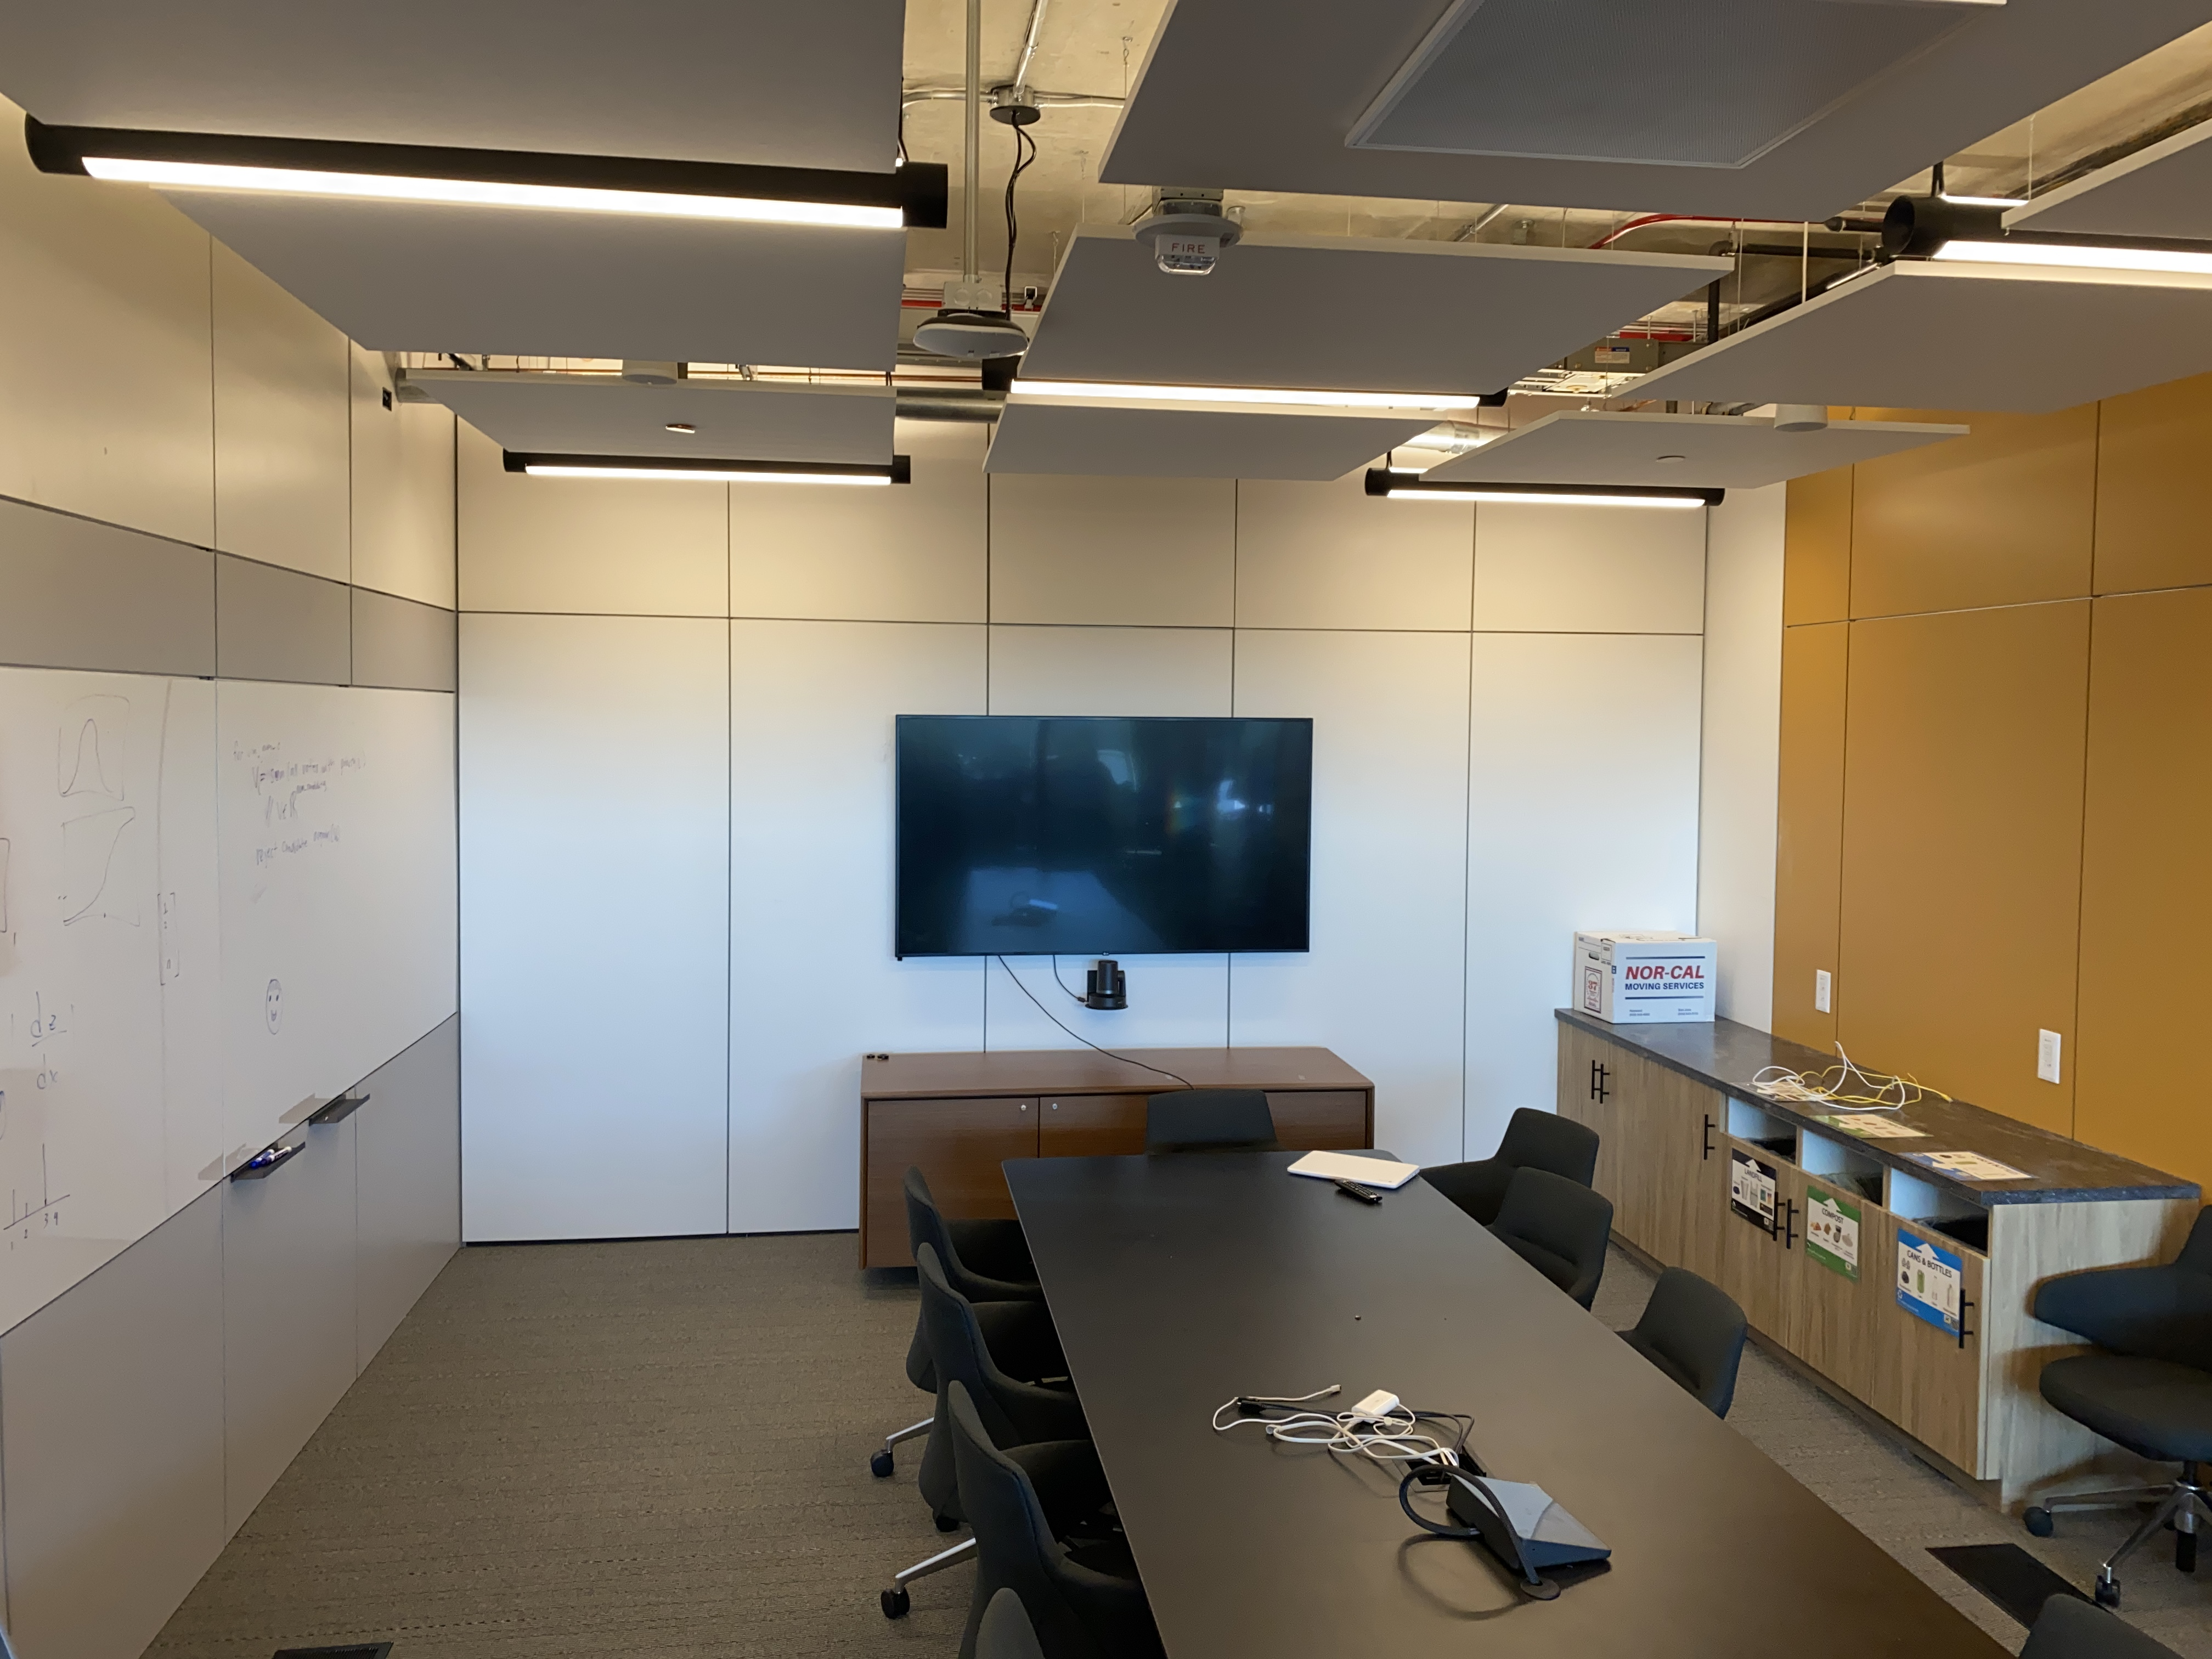
\includegraphics[width=\linewidth]{images/room.jpg}
            \caption{Original Image}
        \end{subfigure}
        \hfill
        \begin{subfigure}[b]{0.45\linewidth}
            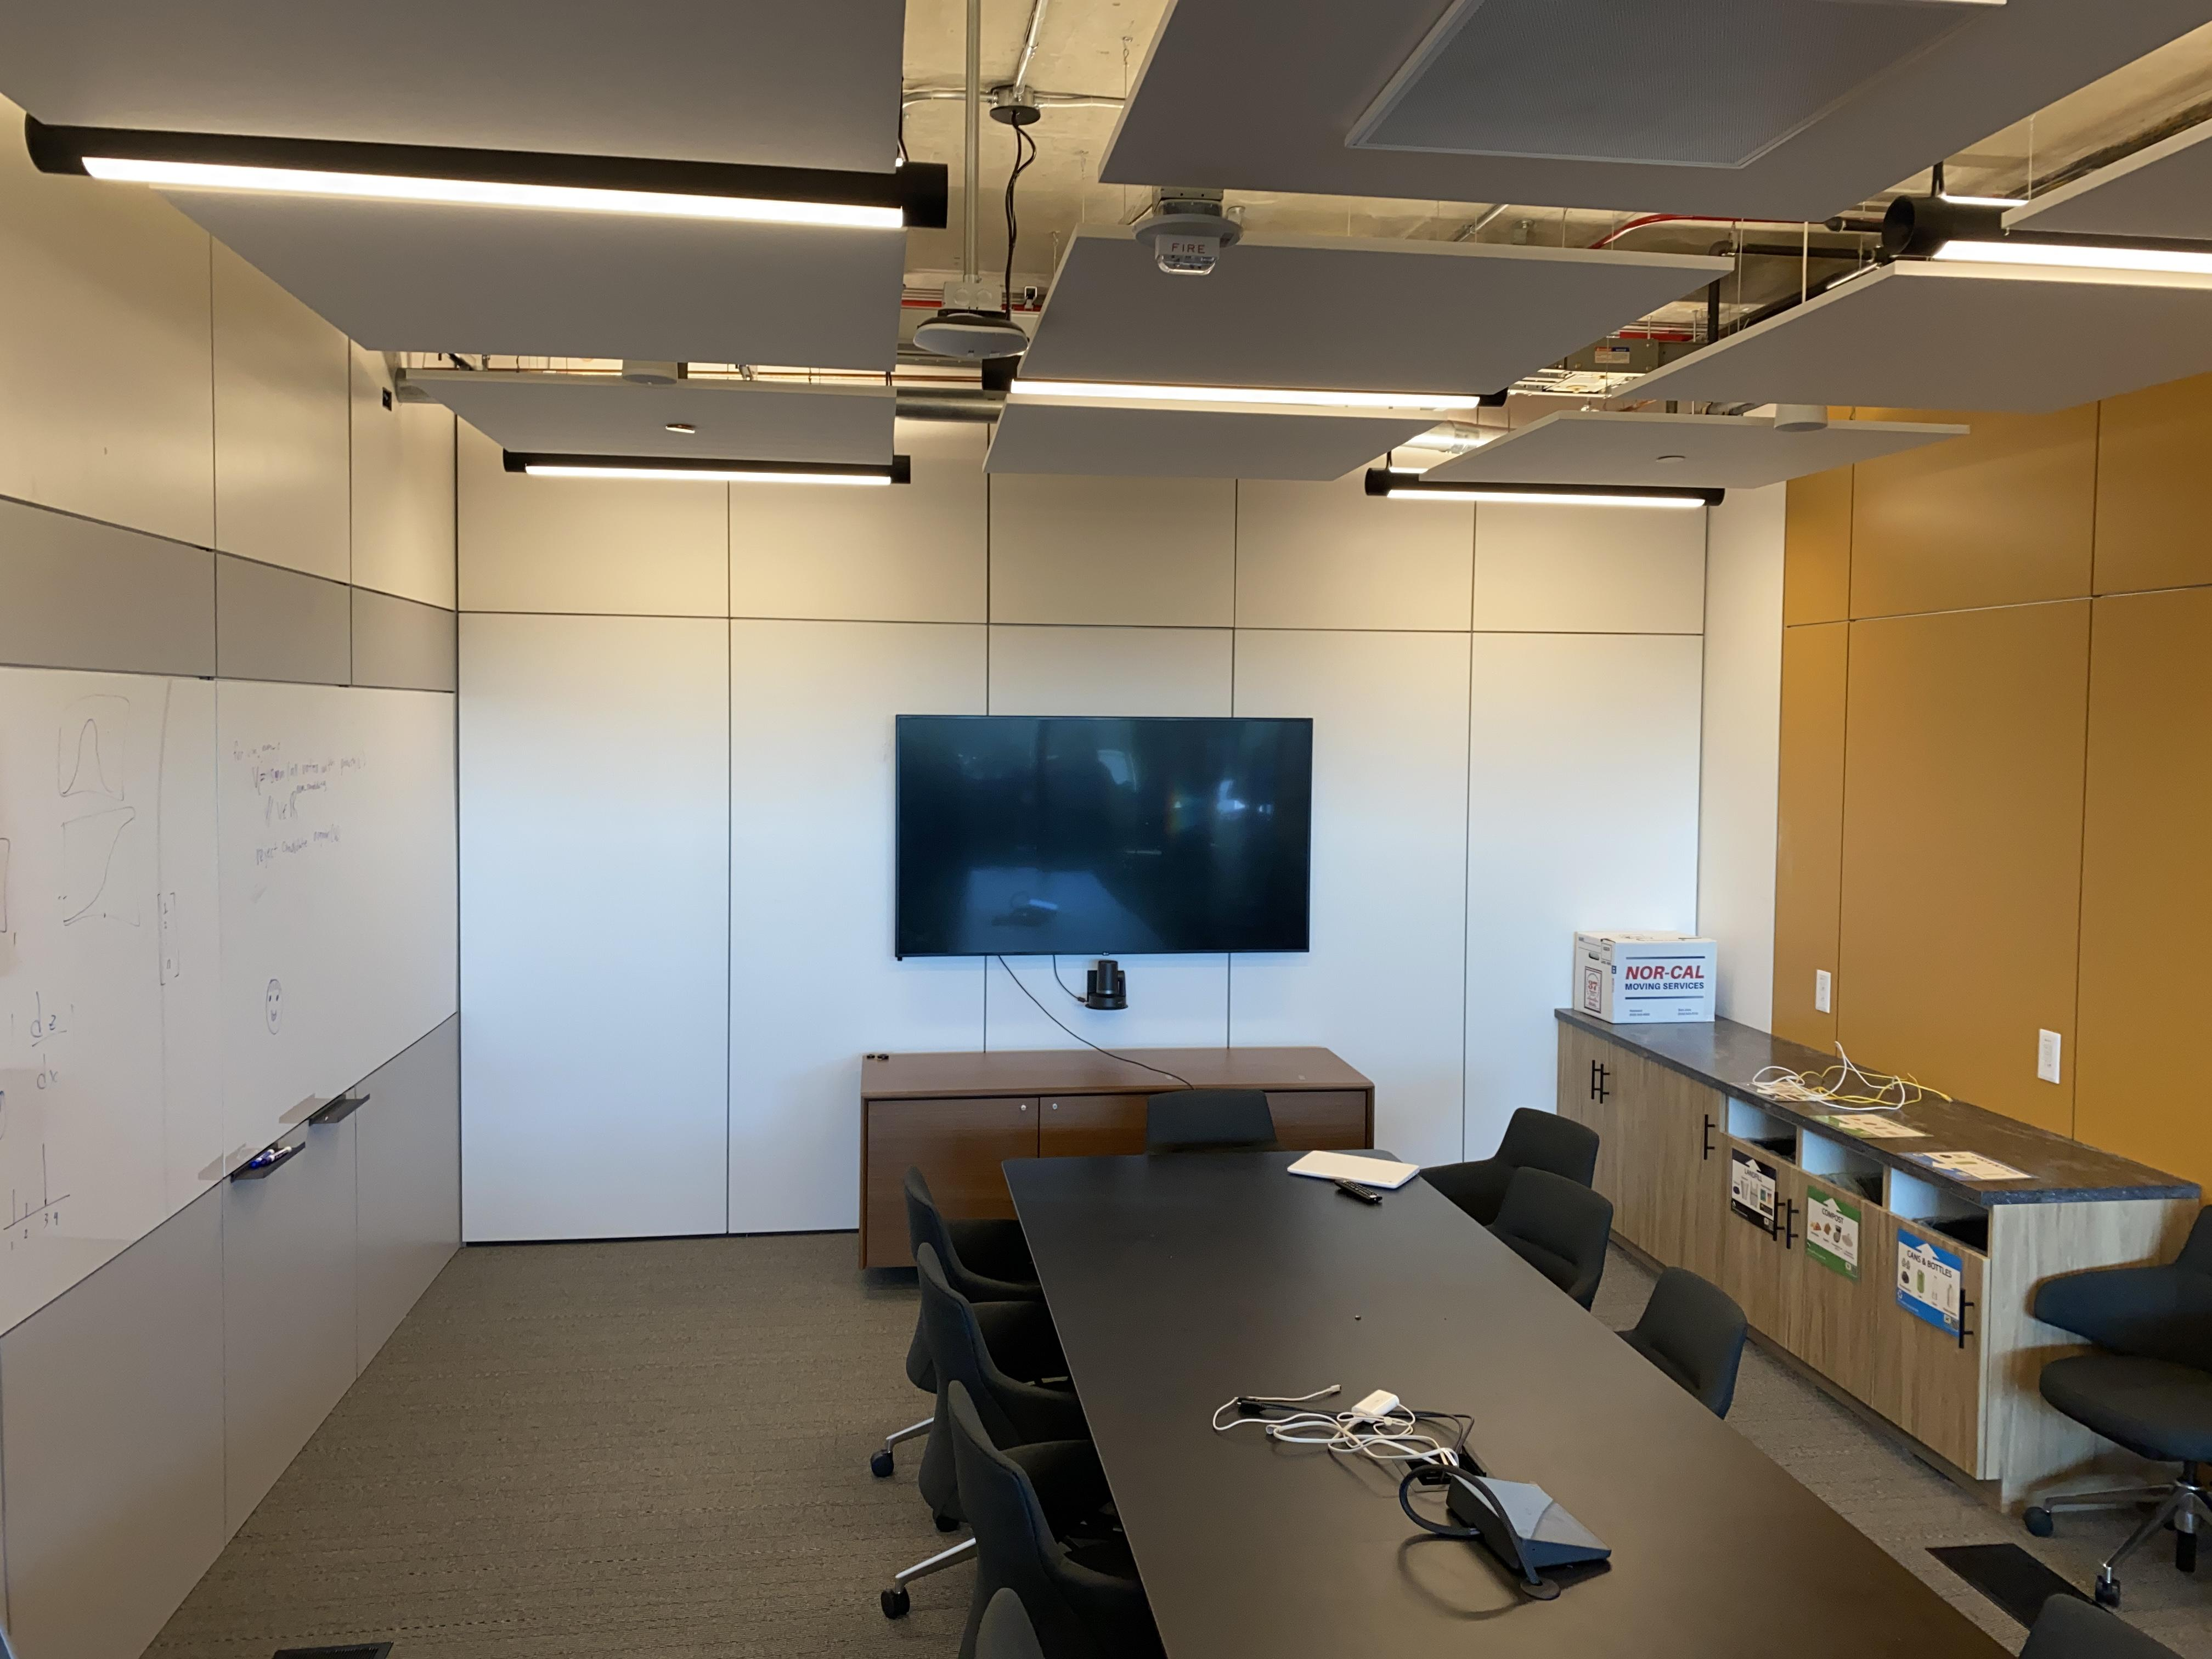
\includegraphics[width=\linewidth]{images/room_recon.jpg}
            \caption{Reconstructed Image}
        \end{subfigure}

        \vspace{0.5cm}
        \begin{subfigure}[b]{0.45\linewidth}
            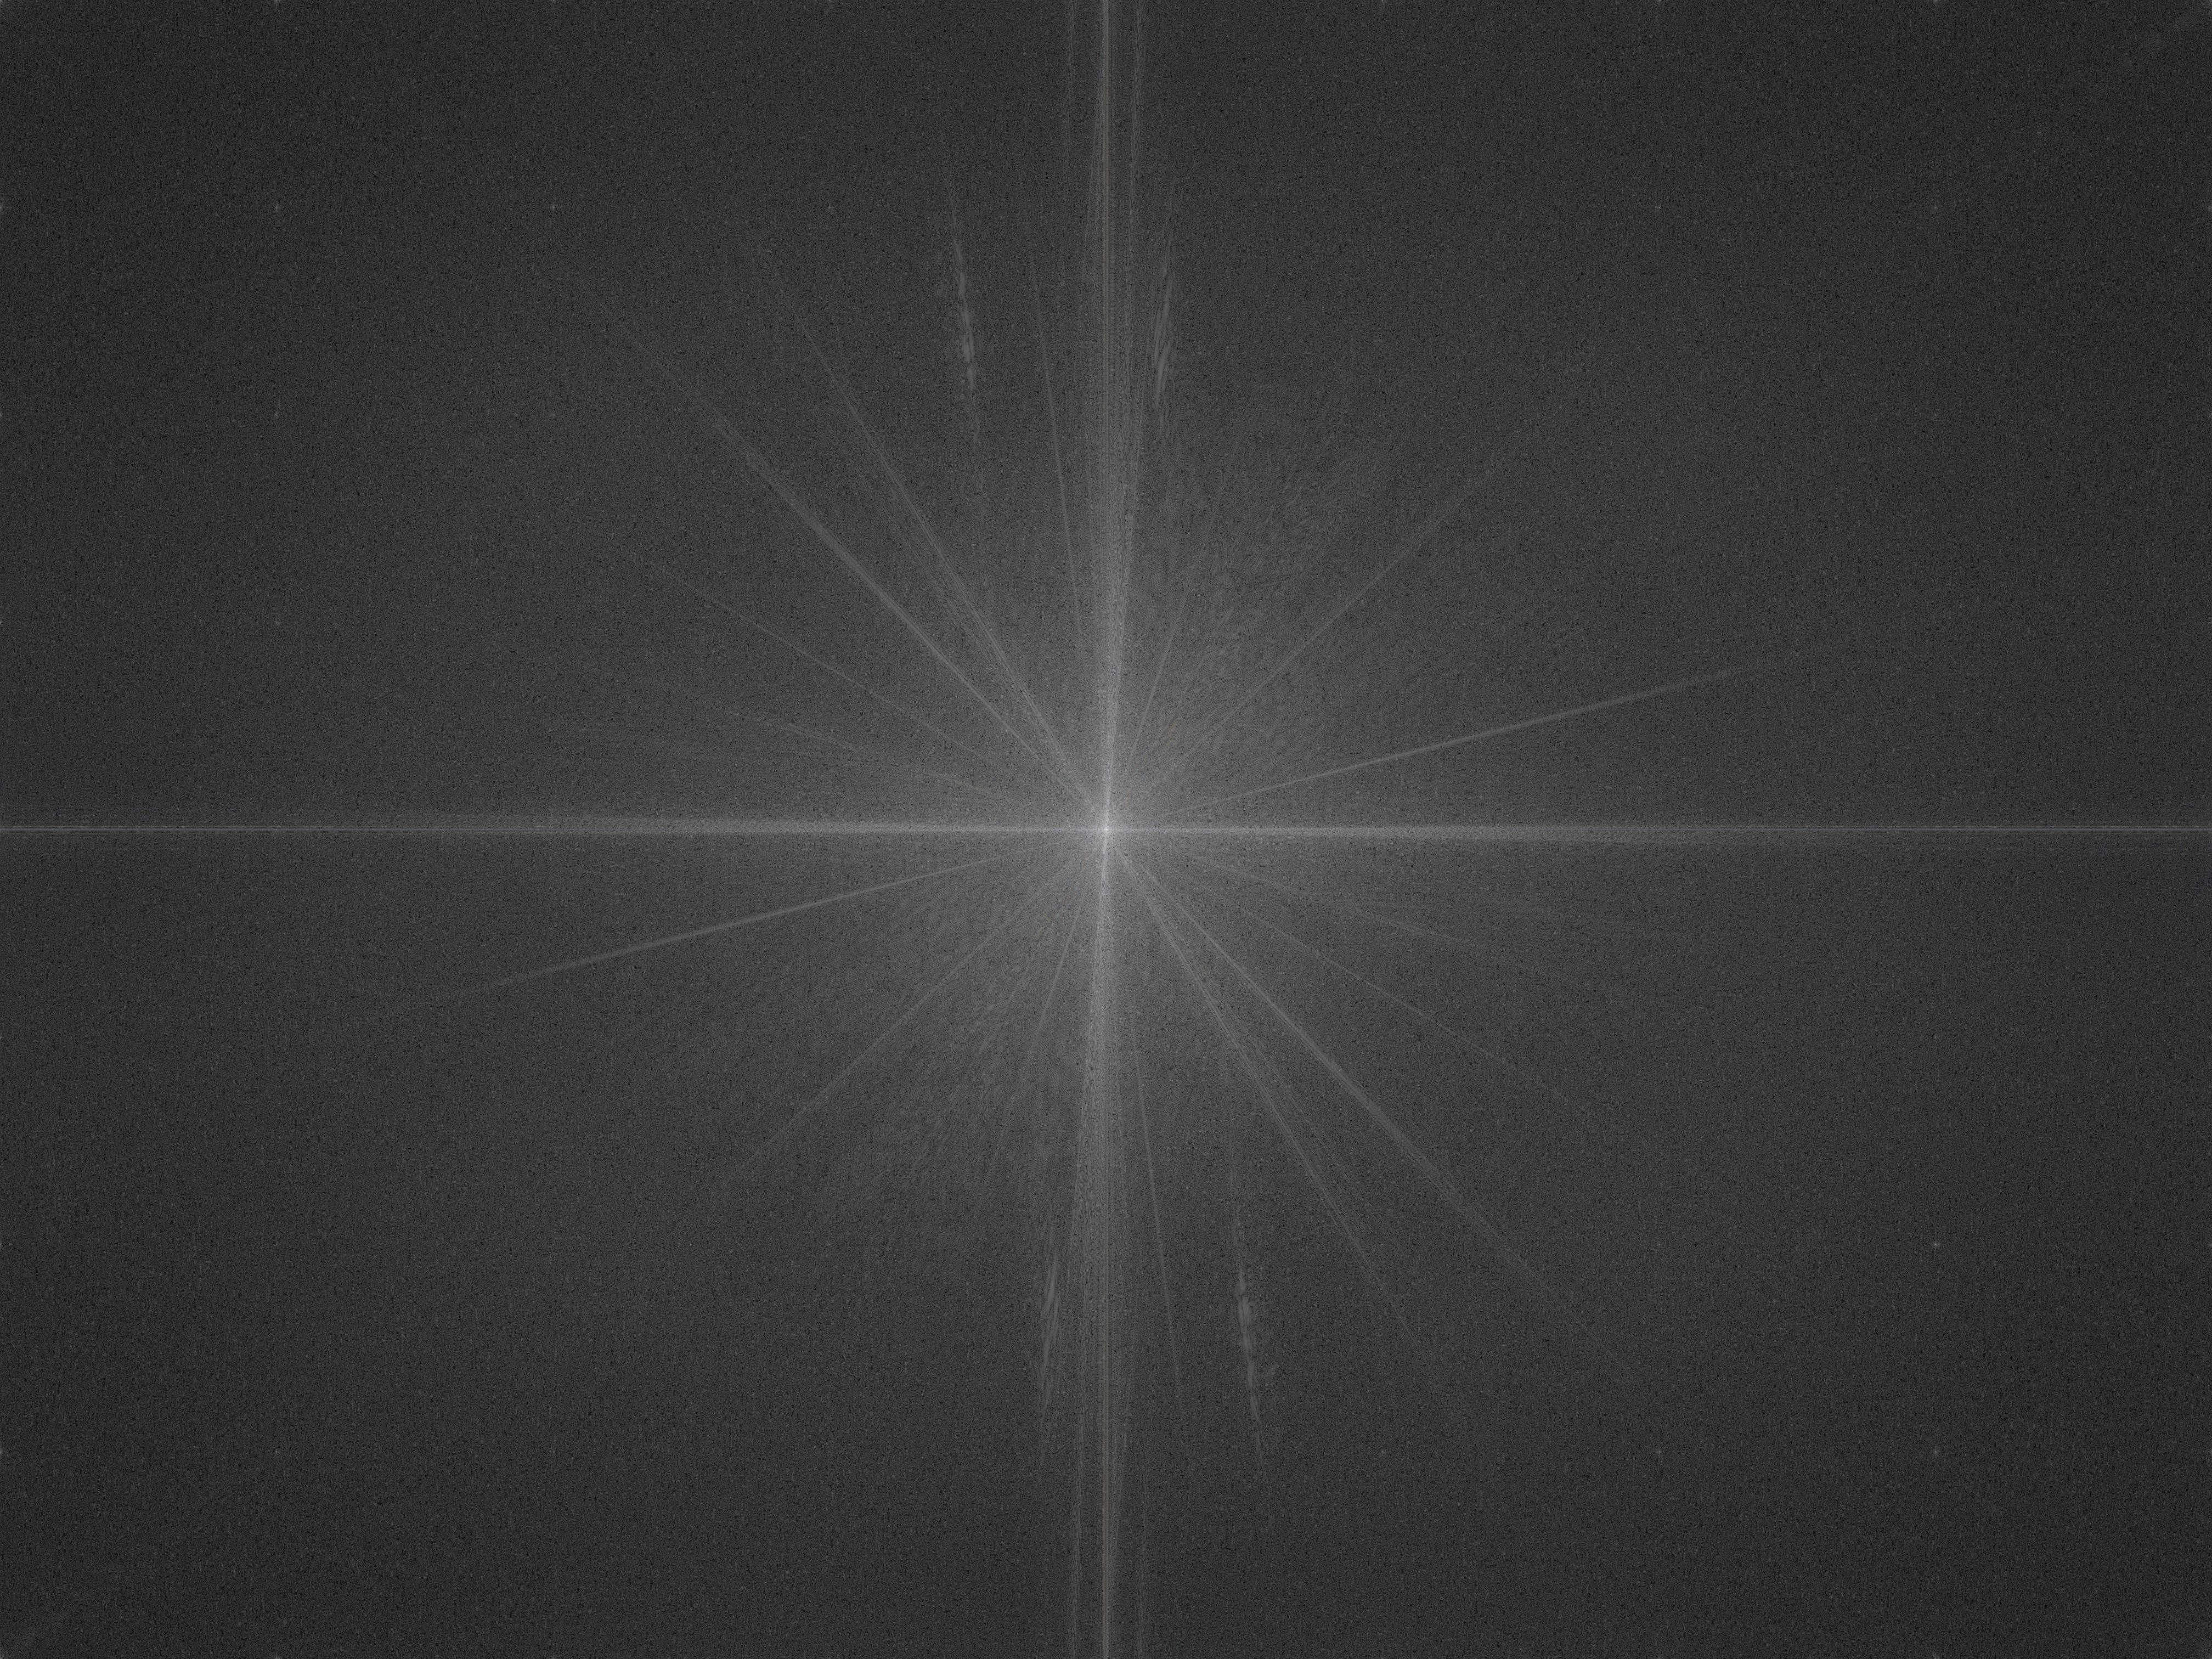
\includegraphics[width=\linewidth]{images/room_magnitude.jpg}
            \caption{Magnitude}
        \end{subfigure}
        \hfill
        \begin{subfigure}[b]{0.45\linewidth}
            \includegraphics[width=\linewidth]{images/room_phase.jpg}
            \caption{Phase}
        \end{subfigure}

        \vspace{0.5cm}
        \begin{subfigure}[b]{0.45\linewidth}
            \includegraphics[width=\linewidth]{images/room_real.jpg}
            \caption{Real Part}
        \end{subfigure}
        \hfill
        \begin{subfigure}[b]{0.45\linewidth}
            \includegraphics[width=\linewidth]{images/room_imag.jpg}
            \caption{Imaginary Part}
        \end{subfigure}

        \caption{Room: Images generated during the DFT process}
        \label{fig:room}
    \end{minipage}
\end{figure}


\begin{figure}[htbp]
    \centering 
    \begin{minipage}{0.8\textwidth} 
        \centering 
        
        \begin{subfigure}[b]{0.45\linewidth} 
            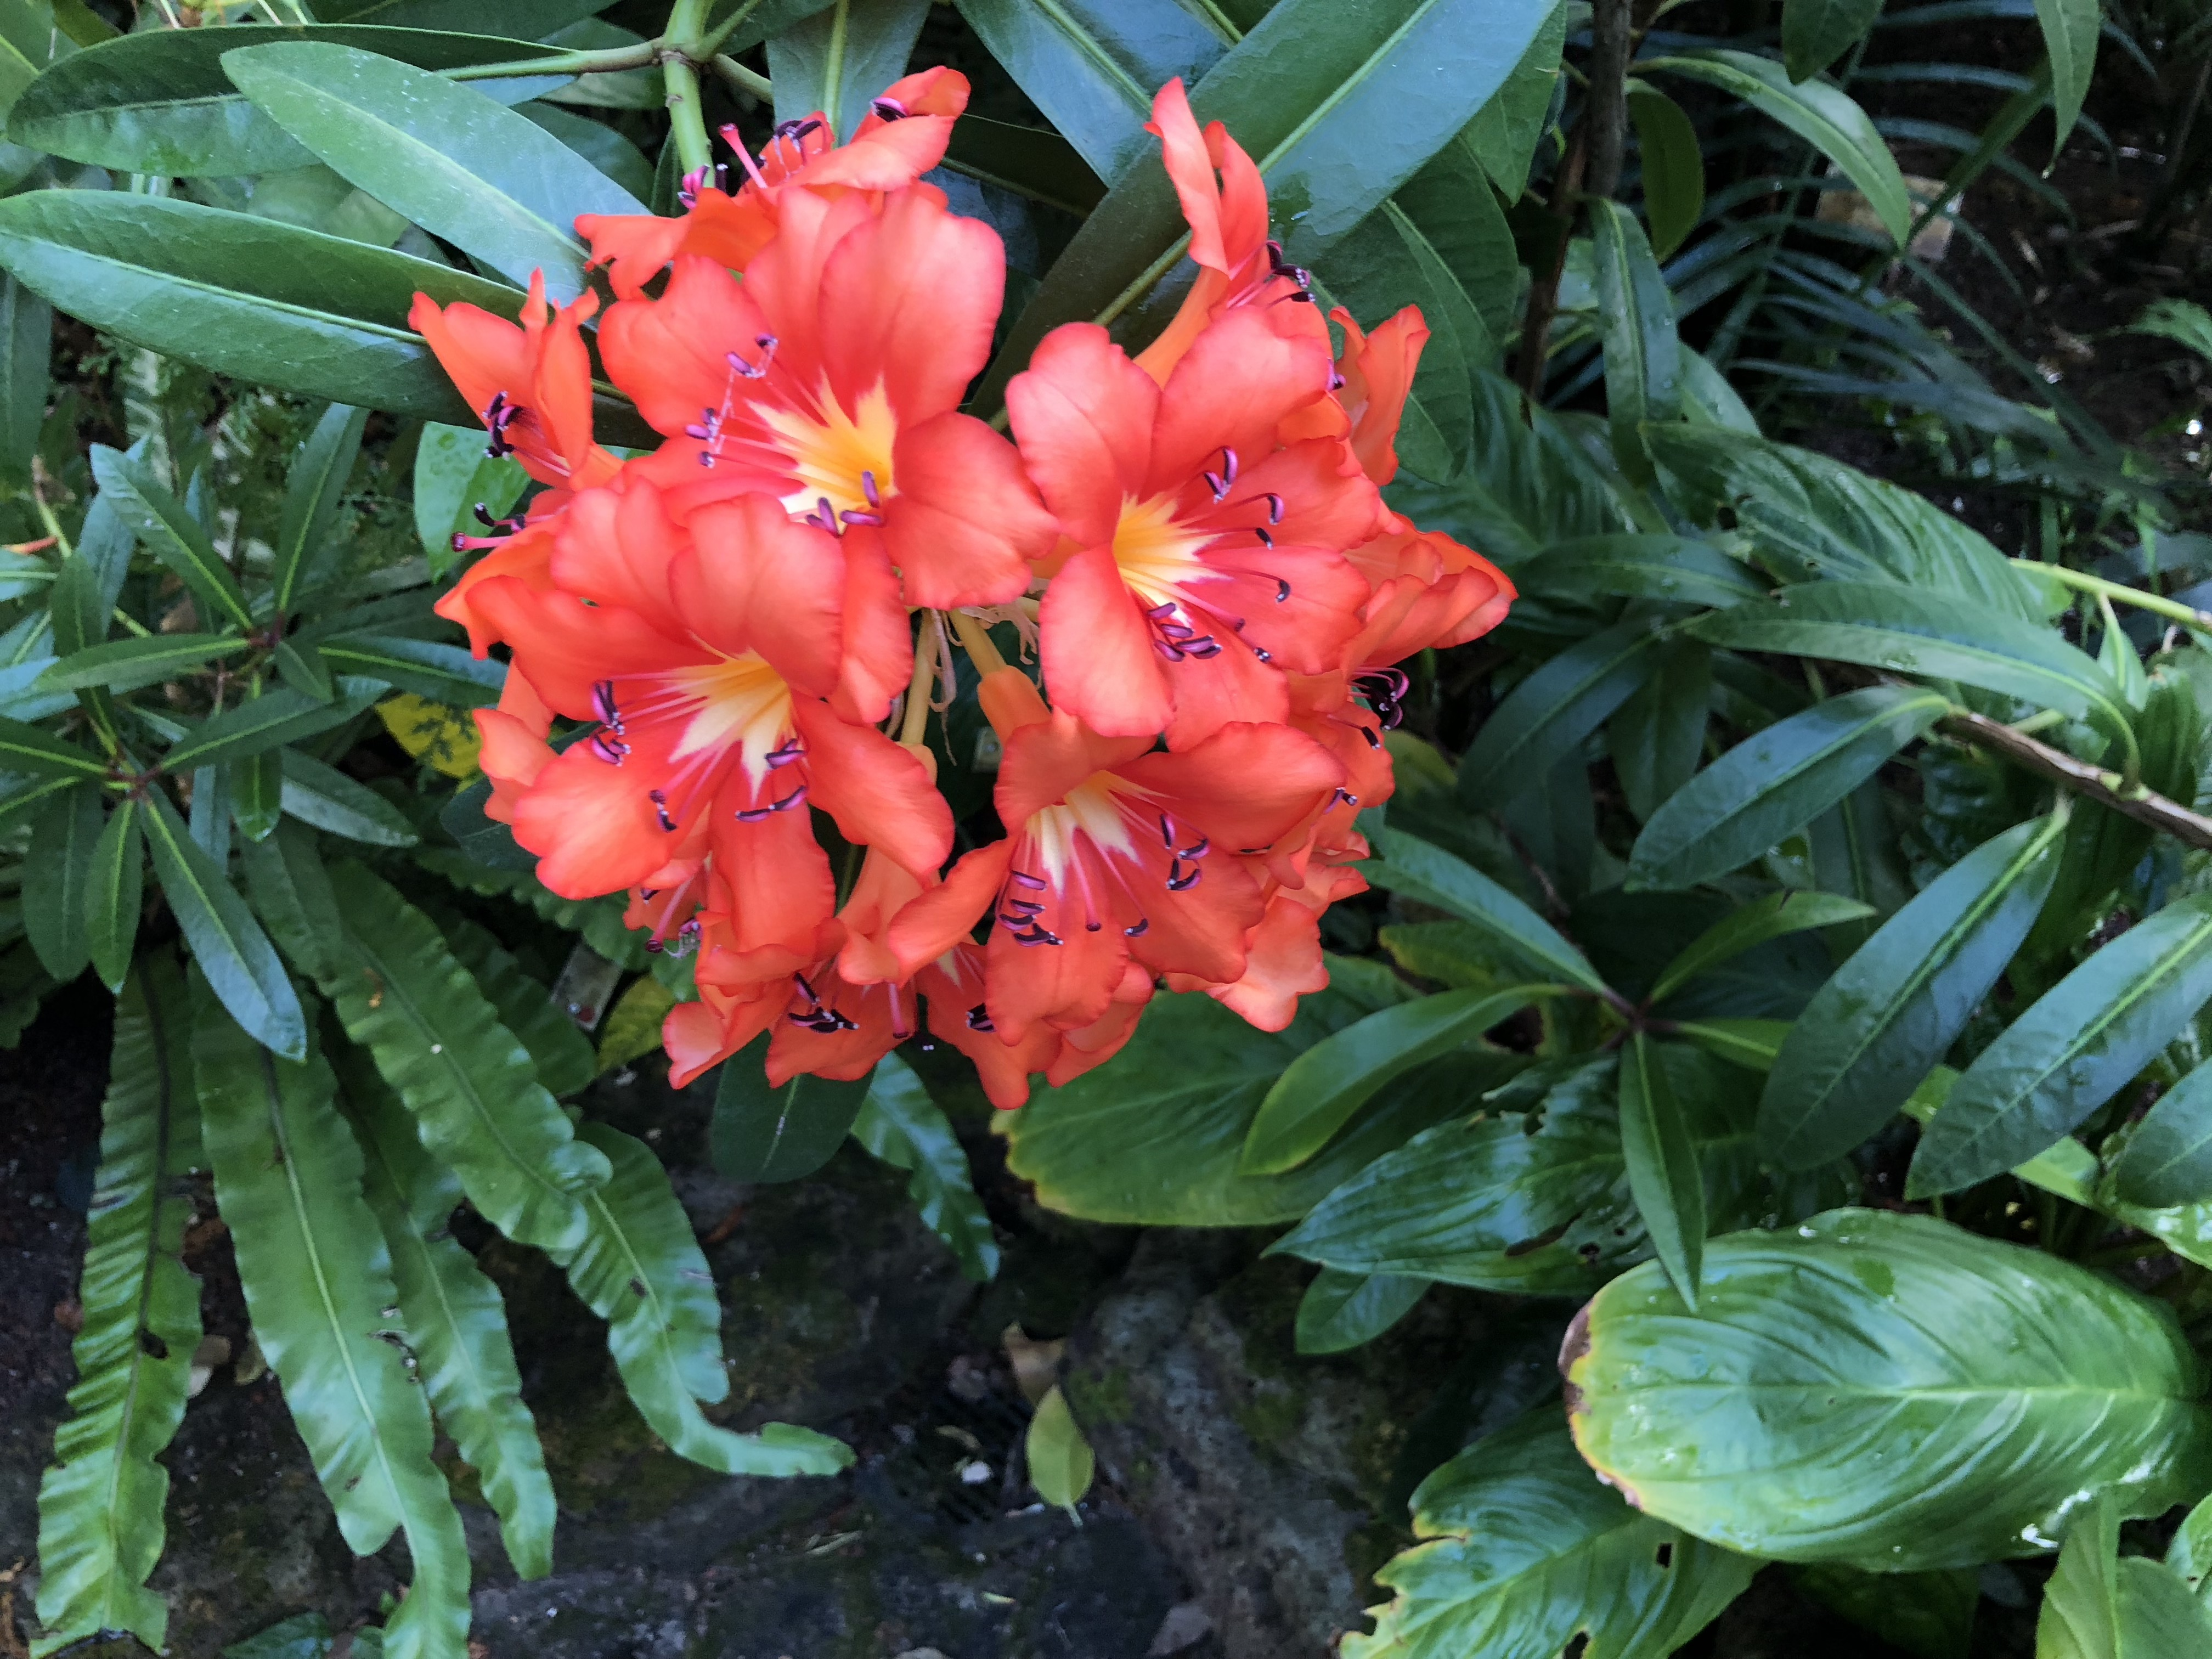
\includegraphics[width=\linewidth]{images/flower.jpg}
            \caption{Original Image}
        \end{subfigure}
        \hfill
        \begin{subfigure}[b]{0.45\linewidth}
            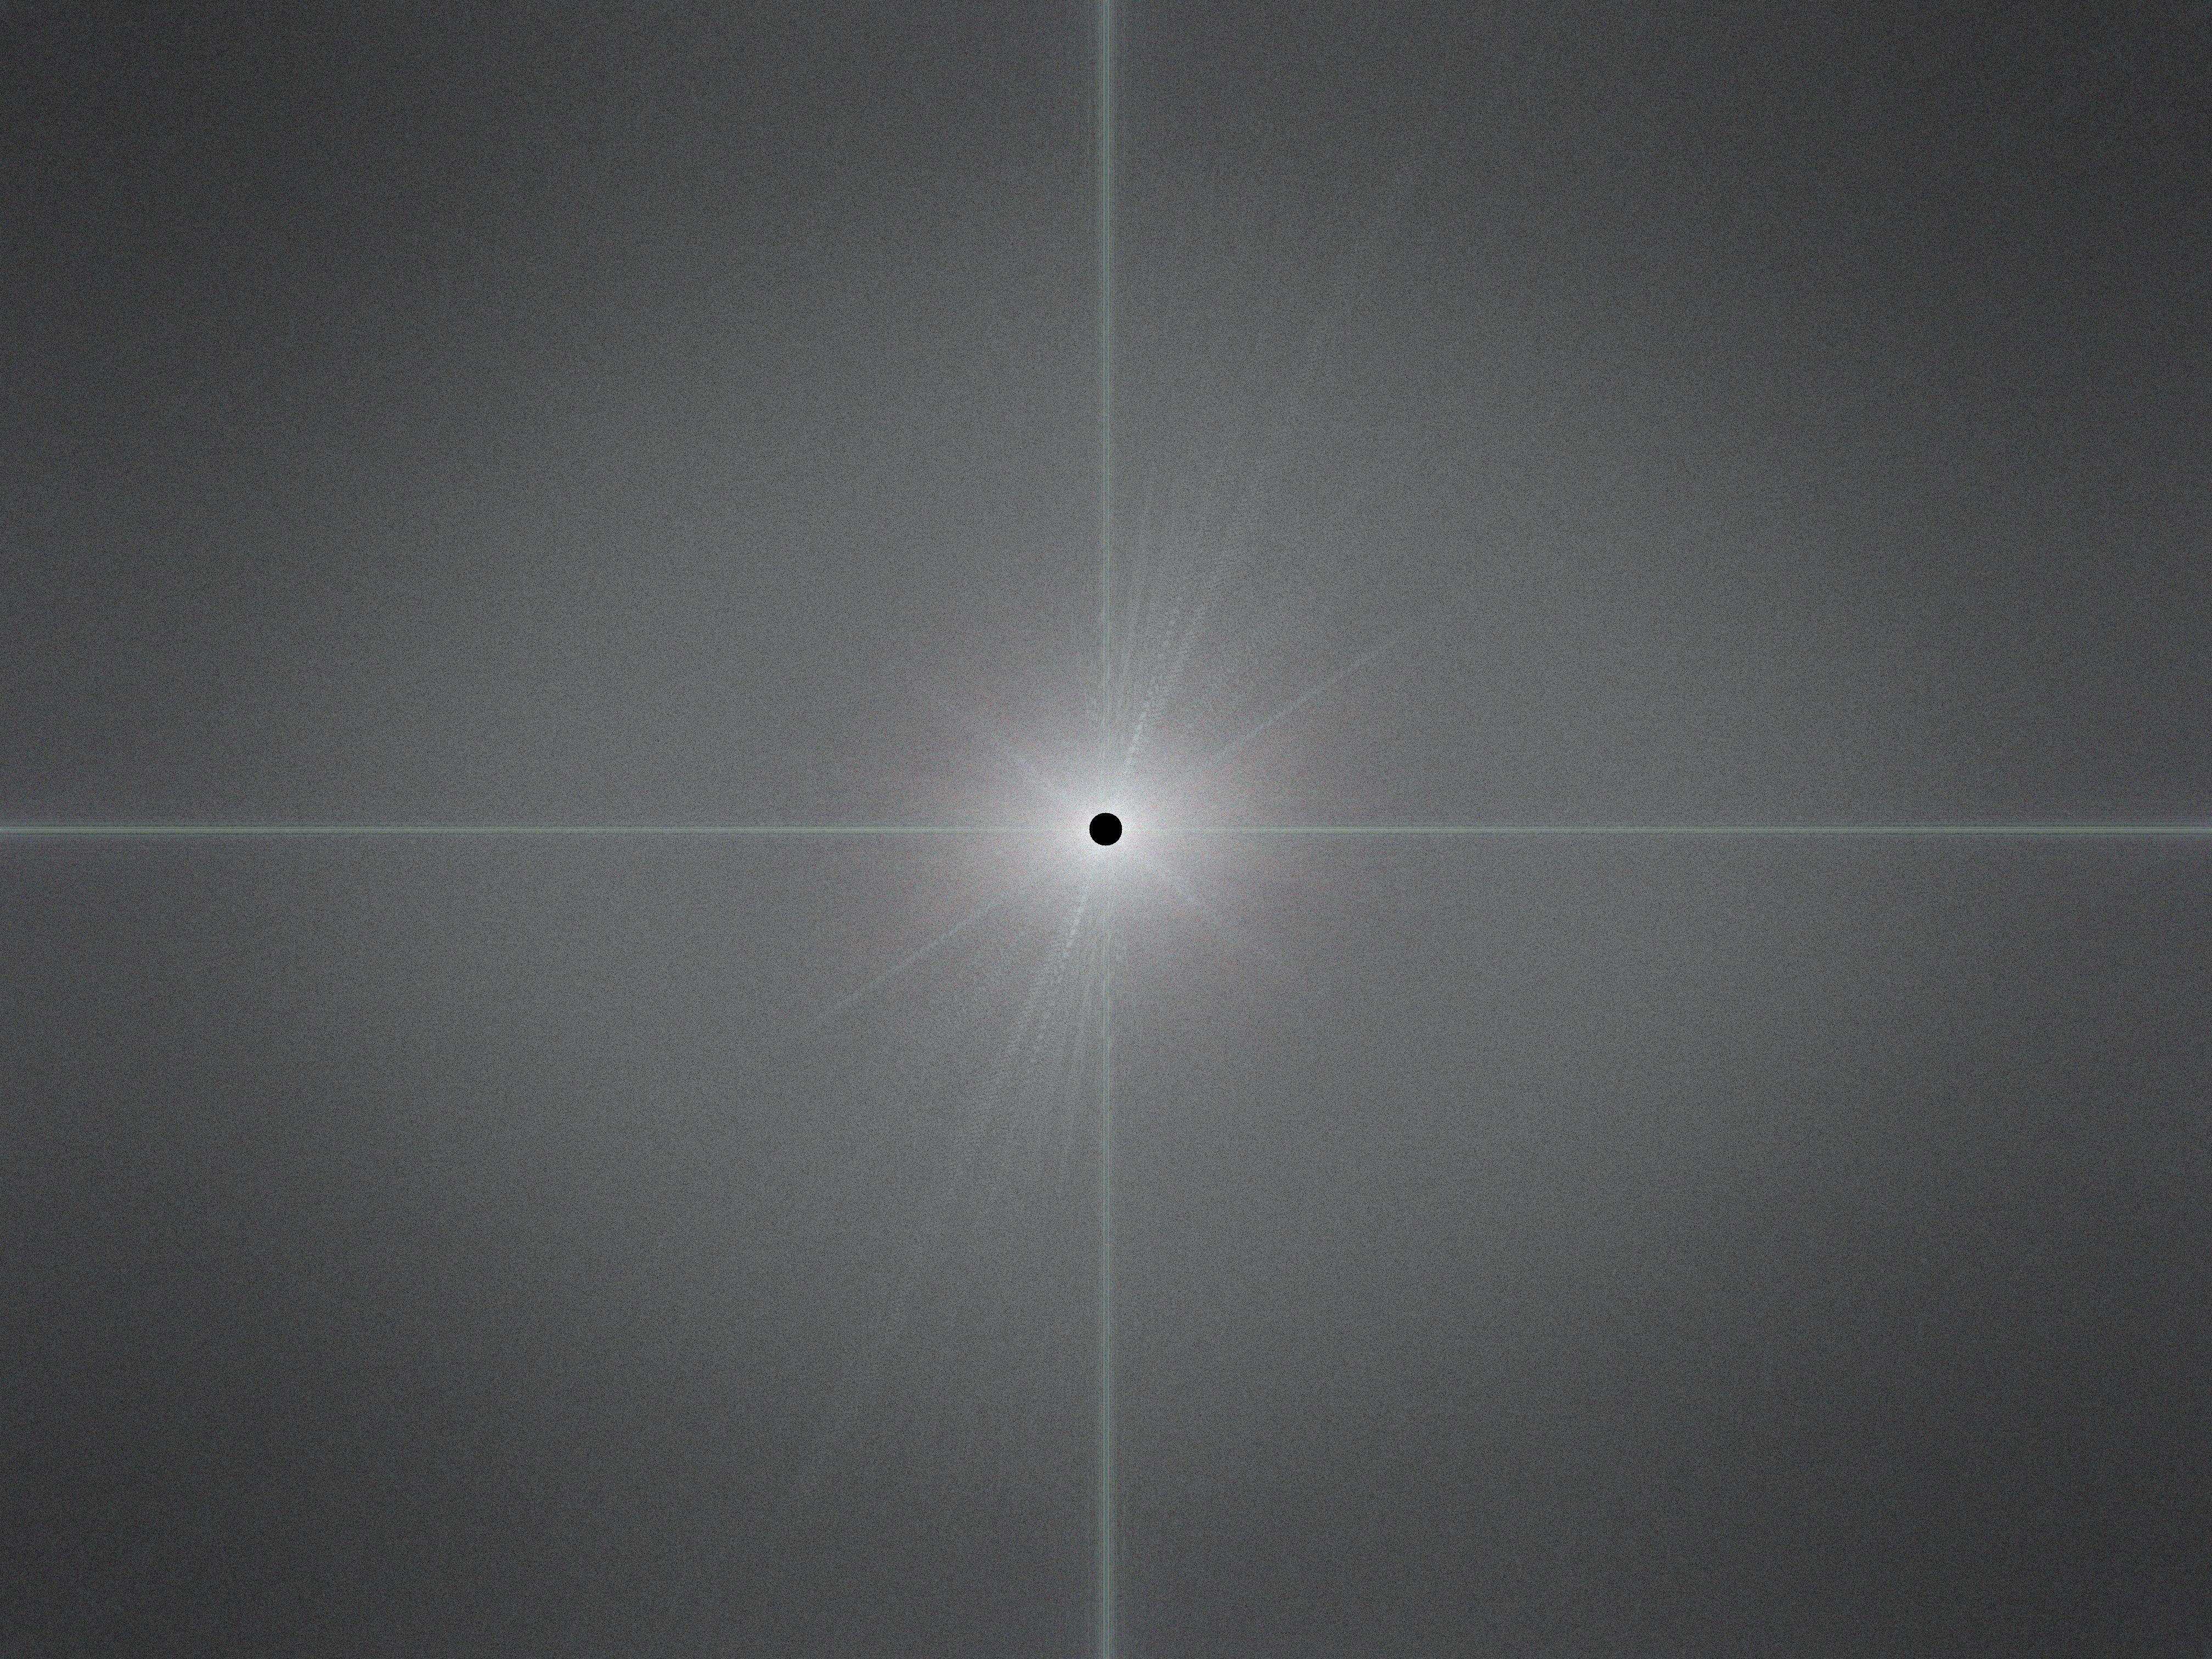
\includegraphics[width=\linewidth]{images/flower_mag_high_30.jpg}
            \caption{High-pass Filter}
        \end{subfigure}

        \vspace{0.5cm}
        \begin{subfigure}[b]{0.45\linewidth}
            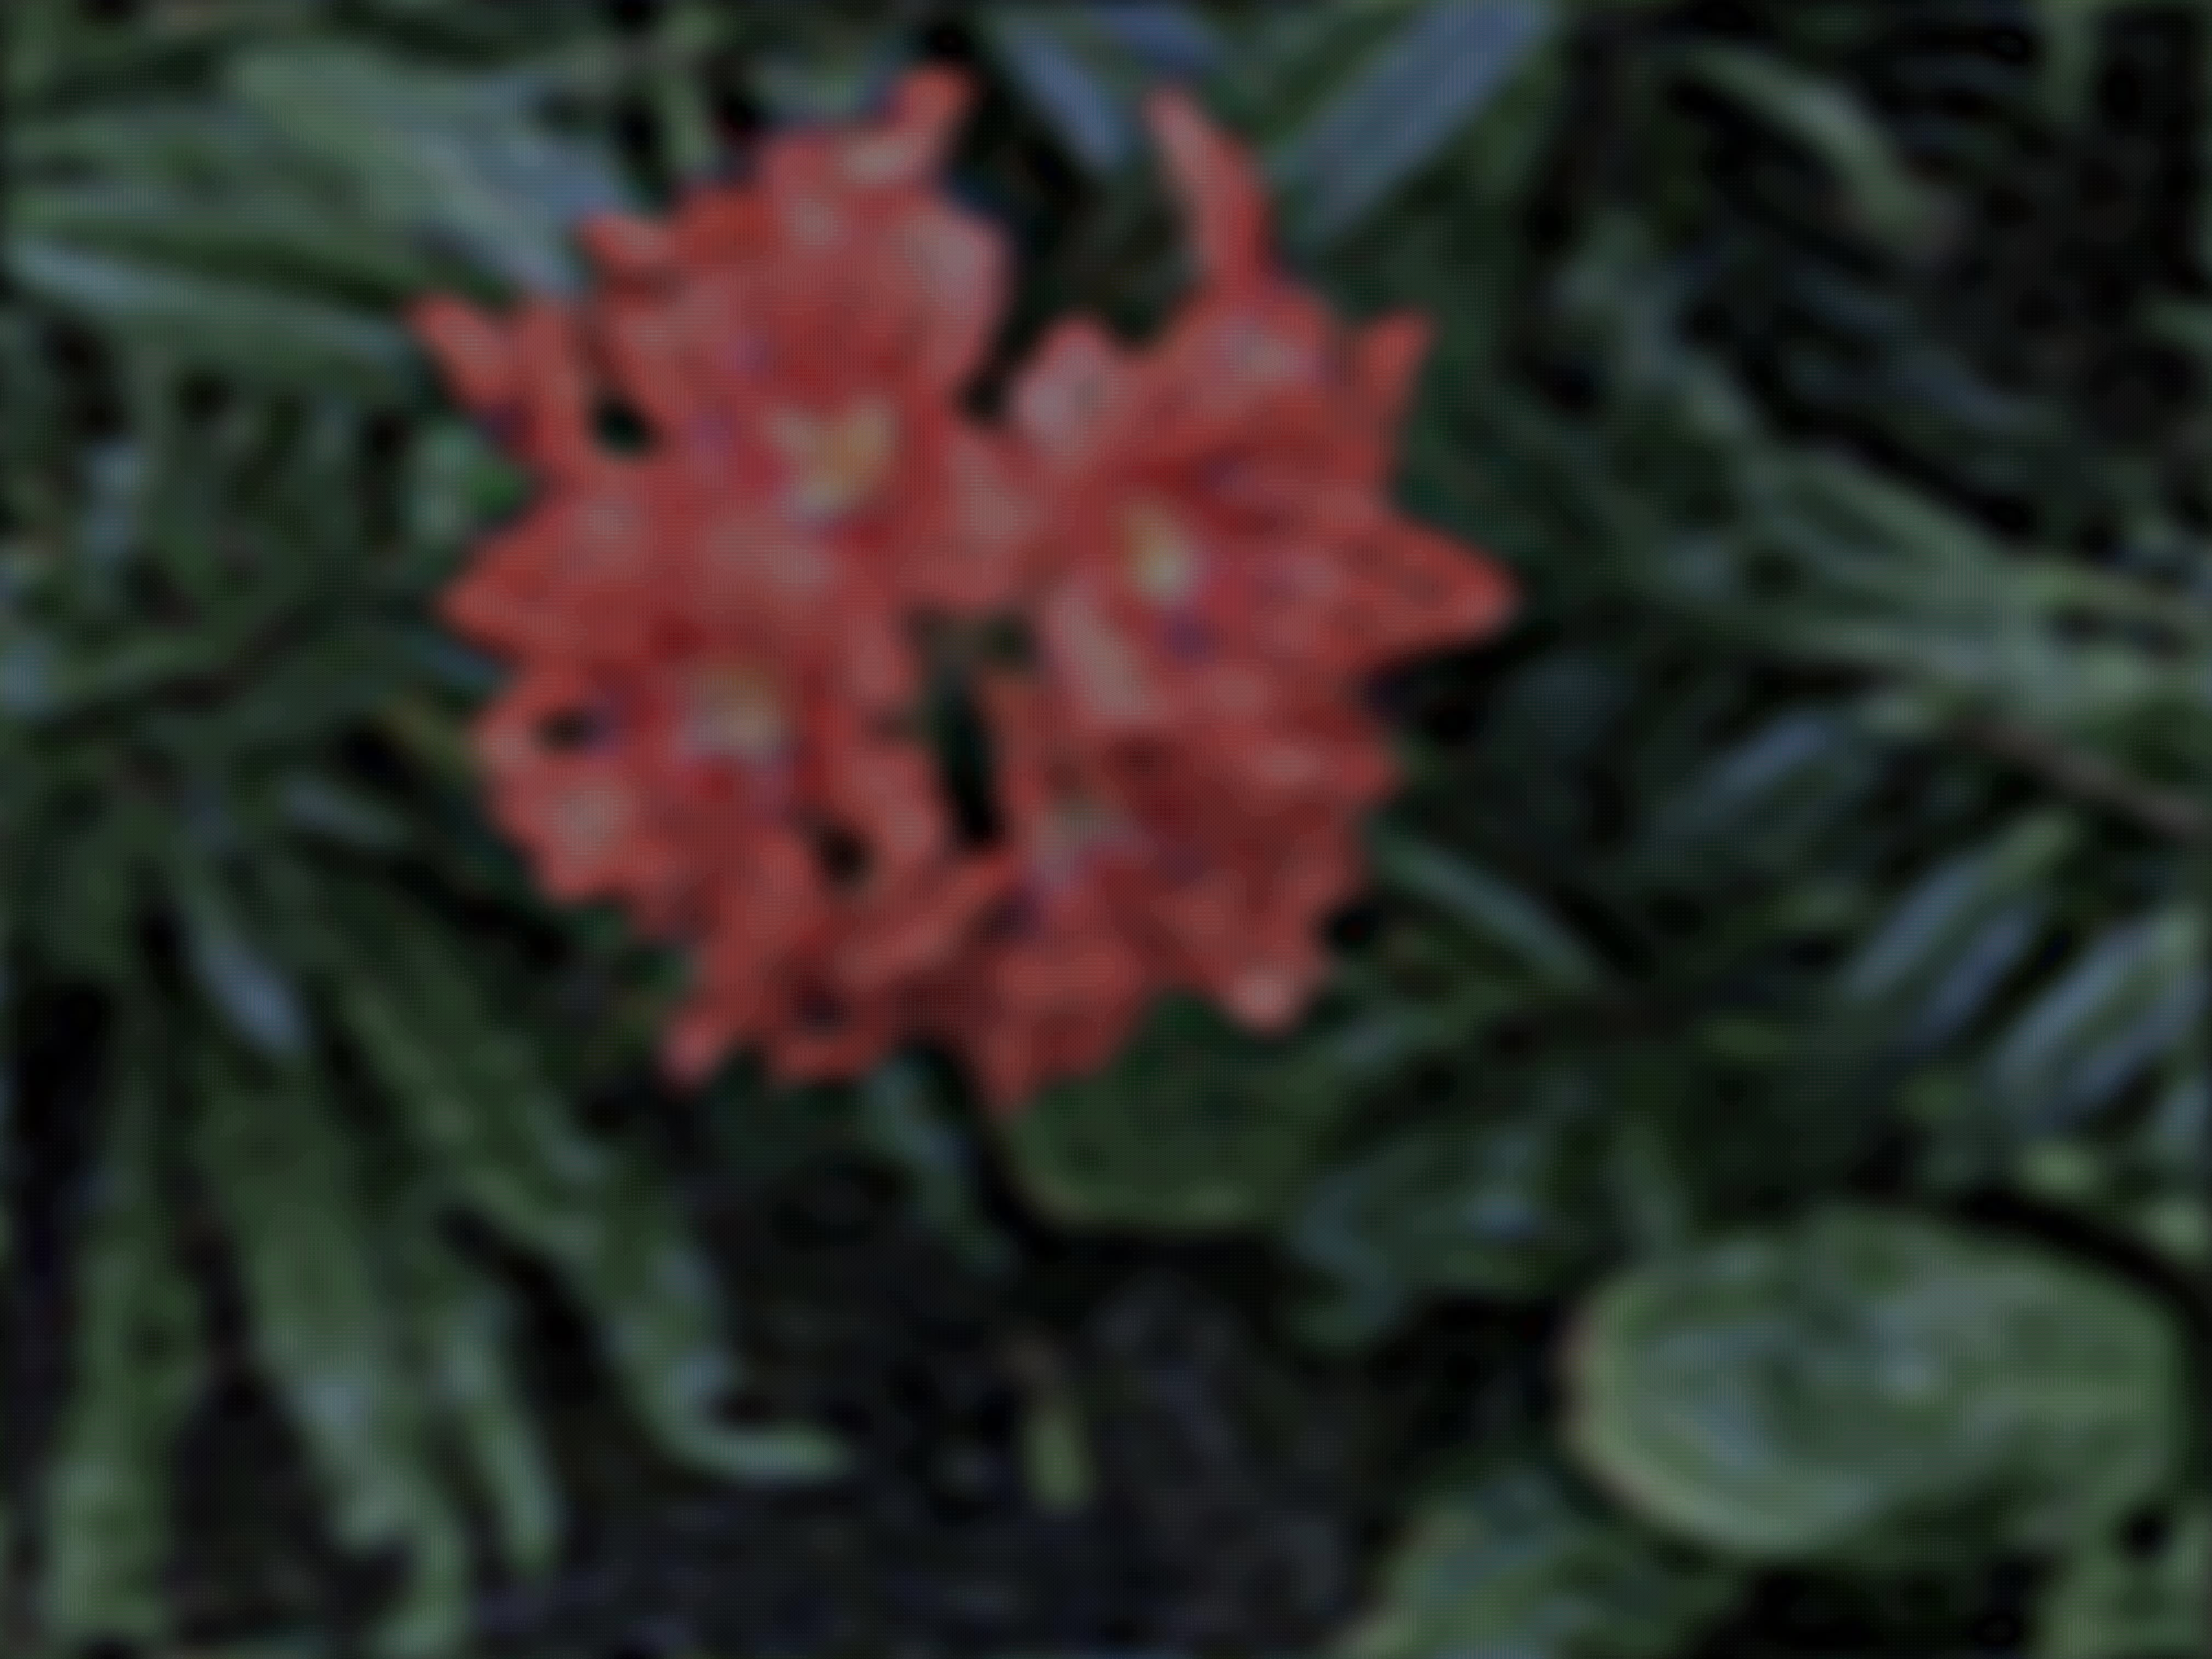
\includegraphics[width=\linewidth]{images/flower_low_30.jpg}
            \caption{Low-pass Image}
        \end{subfigure}
        \hfill
        \begin{subfigure}[b]{0.45\linewidth}
            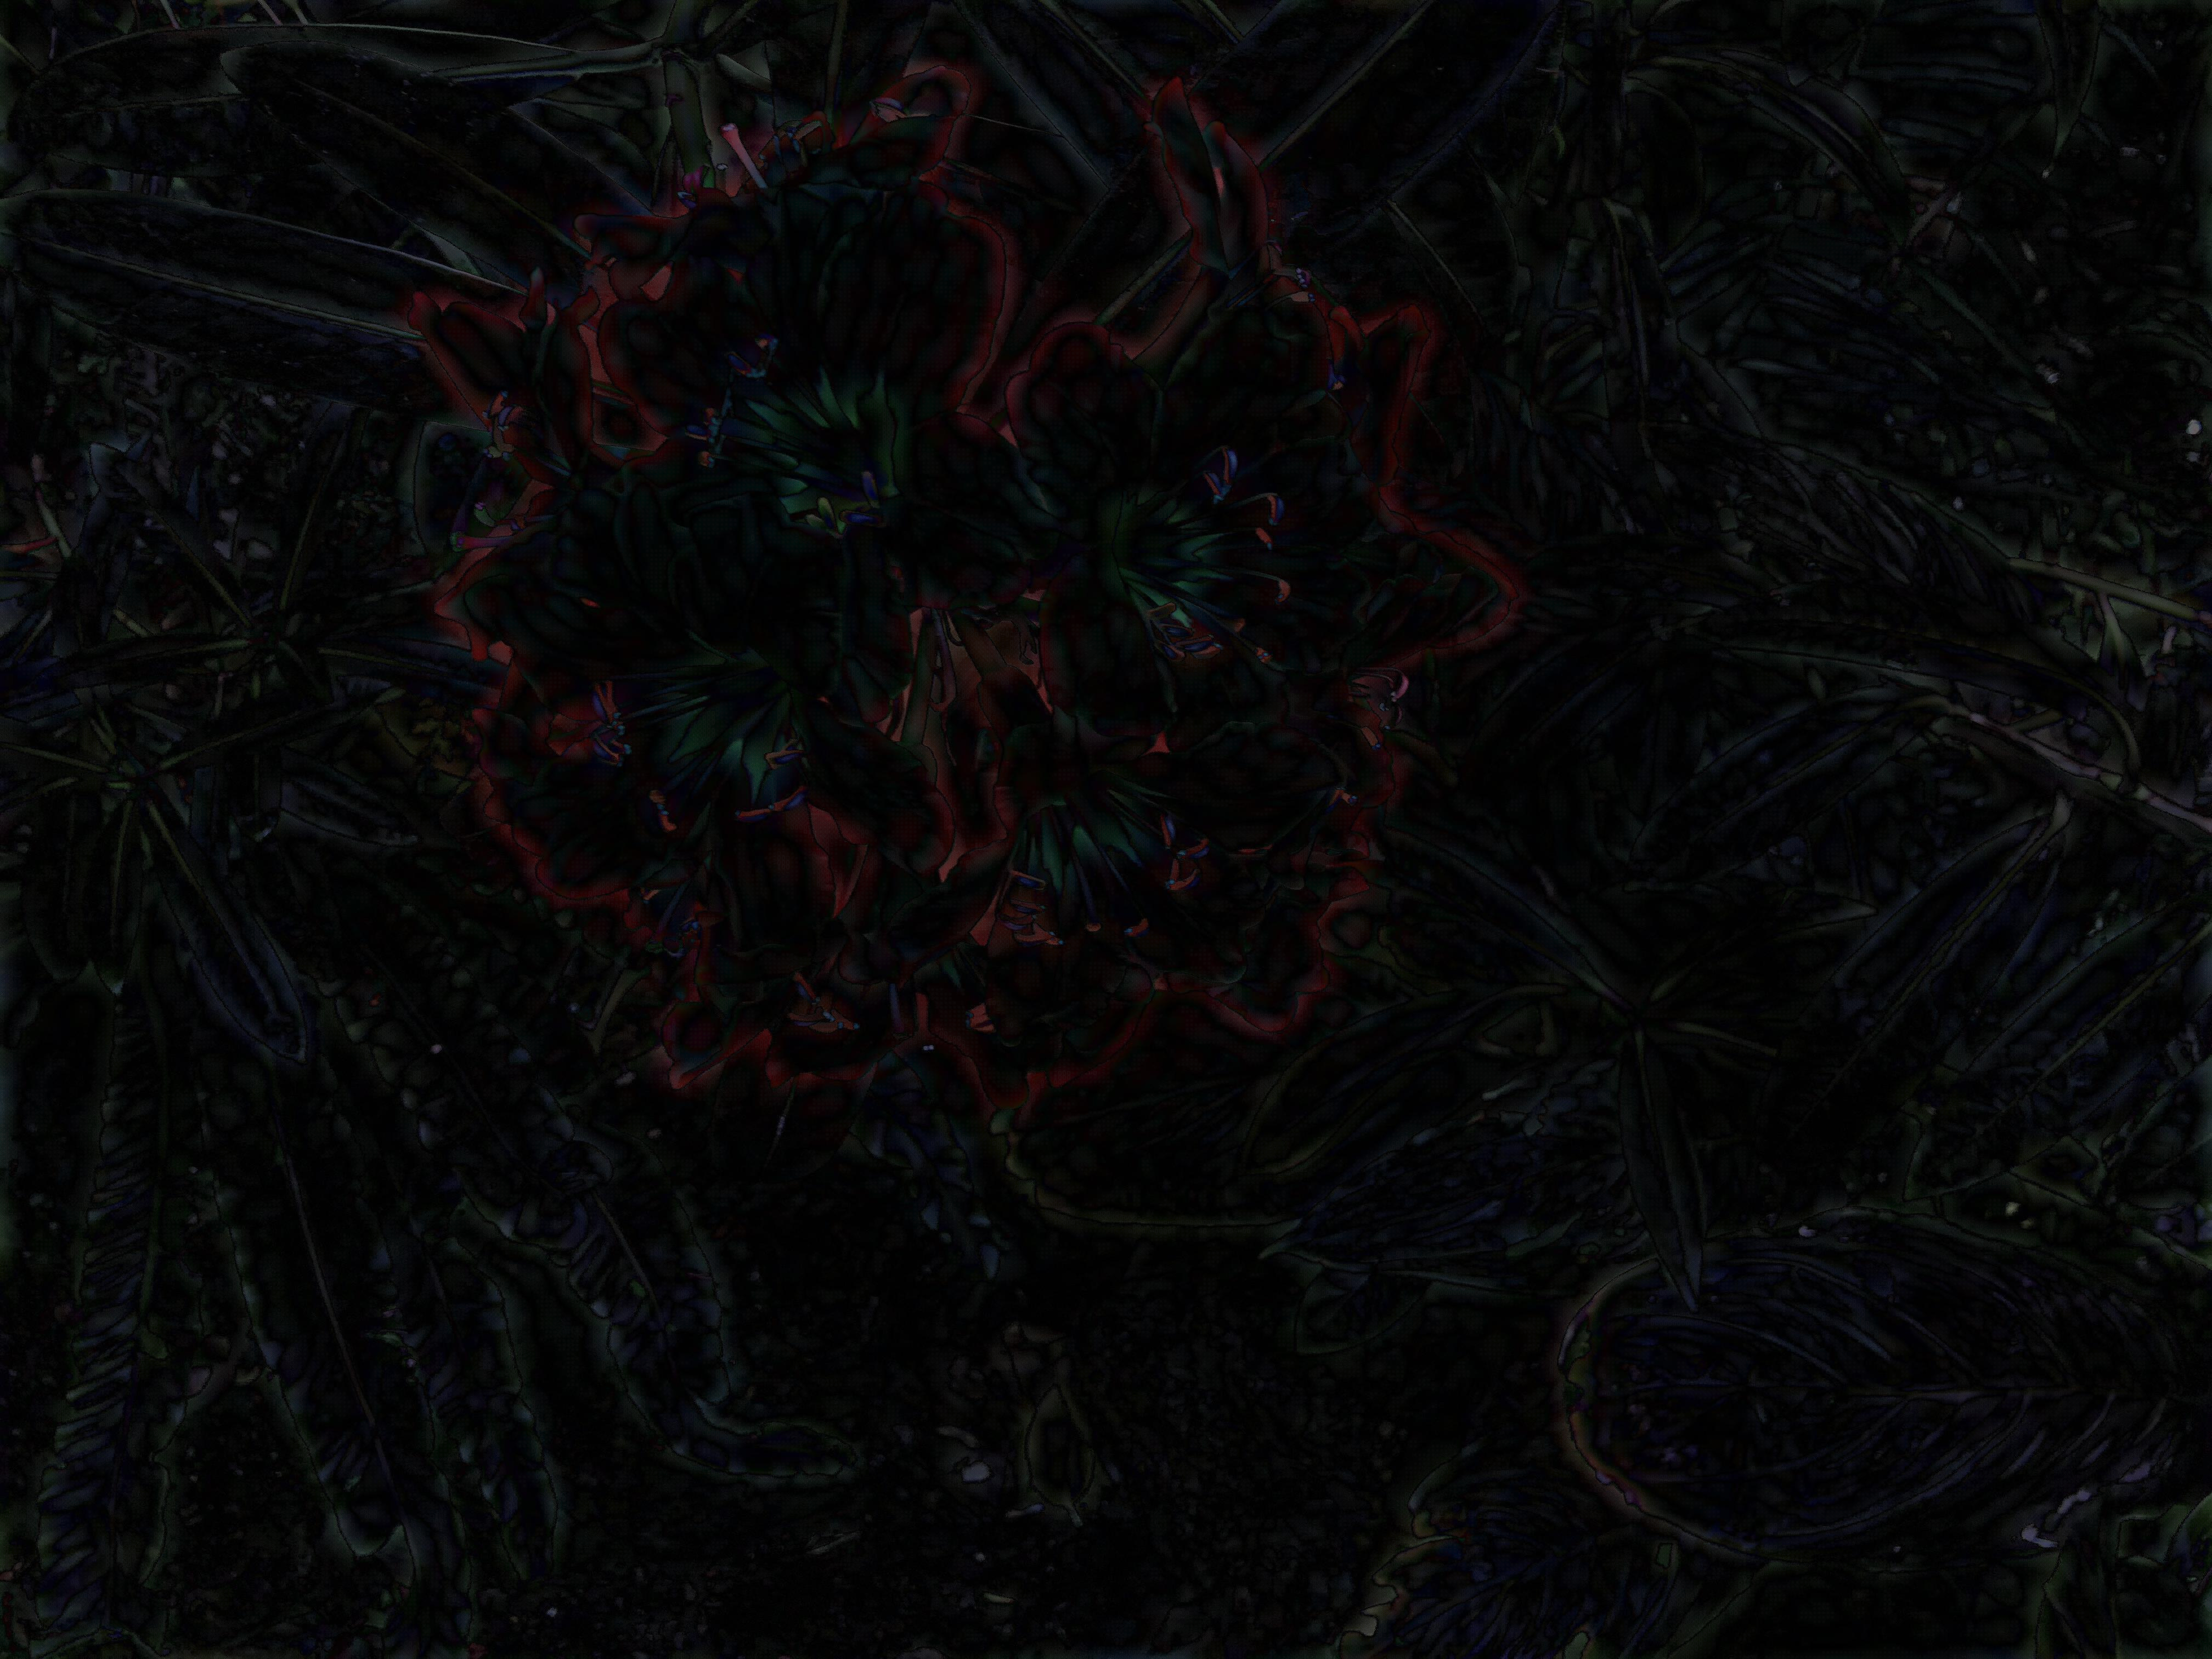
\includegraphics[width=\linewidth]{images/flower_high_30.jpg}
            \caption{High-pass Image}
        \end{subfigure}

        \caption{Flower: Comparison between the Original and Filtered Images with D0=30}
        \label{fig:flower}
    \end{minipage}
\end{figure}



\begin{problem}{Result Analysis}{result}

\begin{enumerate}[(a)]
    \item \textbf{Reconstructed and Filtered Images}
    
    Figure \ref{fig:room} and \ref{fig:flower} respectively show the reconstructed image and the high/low-pass image. i) The reconstruction result is satisfactory, as no obvious distinction can be noticed, showing that our DFT and IDFT implementation is correct. ii) The high-pass filter succeeds to separate high-frequency components from the low-frequency ones, with the outline of the flower in the high-pass image and the low-pass image becomes blur and reduces noises.
    \item \textbf{Reconstructed Error Evaluation}
    We define the metric below to show the performance of our reconstruction. And results can be found in Table \ref{table:evaluation}. The tiny discrepancy arises from the limited complex calculation precision in DFT and IDFT.
    $$error = \frac{\sum_{(x,y)} \vert img_{ori} - img_{recon}\vert} {MN}$$
\end{enumerate}
\end{problem}

\begin{table}[]
    \centering
    \begin{tabular}{|l|l|l|l|l|}
        \hline
        Image Pairs & Flower & Lena & Room \\ \hline
        Error        & 5.4324e-13  & 7.546e-14     & 6.6642e-13   \\ \hline
          
    \end{tabular}
    \caption{Error evaluation for each original and reconstructed image pair}
    \label{table:evaluation}
\end{table}

\begin{problem}{Appendix: Detailed Experiment Results}{appendix}
    \begin{enumerate}[(a)]
        \item \textbf{Reconstructed Image, Magnitude, Phase, Real Part, Imaginary Part}

        Figure \ref{fig:room}, \ref{fig:flower_1}, \ref{fig:lena_1}
        \item \textbf{High-Pass Filter, High-Pass Image, Low-Pass Image}

        Figure \ref{fig:flower}, \ref{fig:lena_2}, \ref{fig:room_2}
    \end{enumerate}
\end{problem}

\begin{figure}[htbp]
    \centering 
    \begin{minipage}{0.8\textwidth} 
        \centering 
        
        \begin{subfigure}[b]{0.45\linewidth} 
            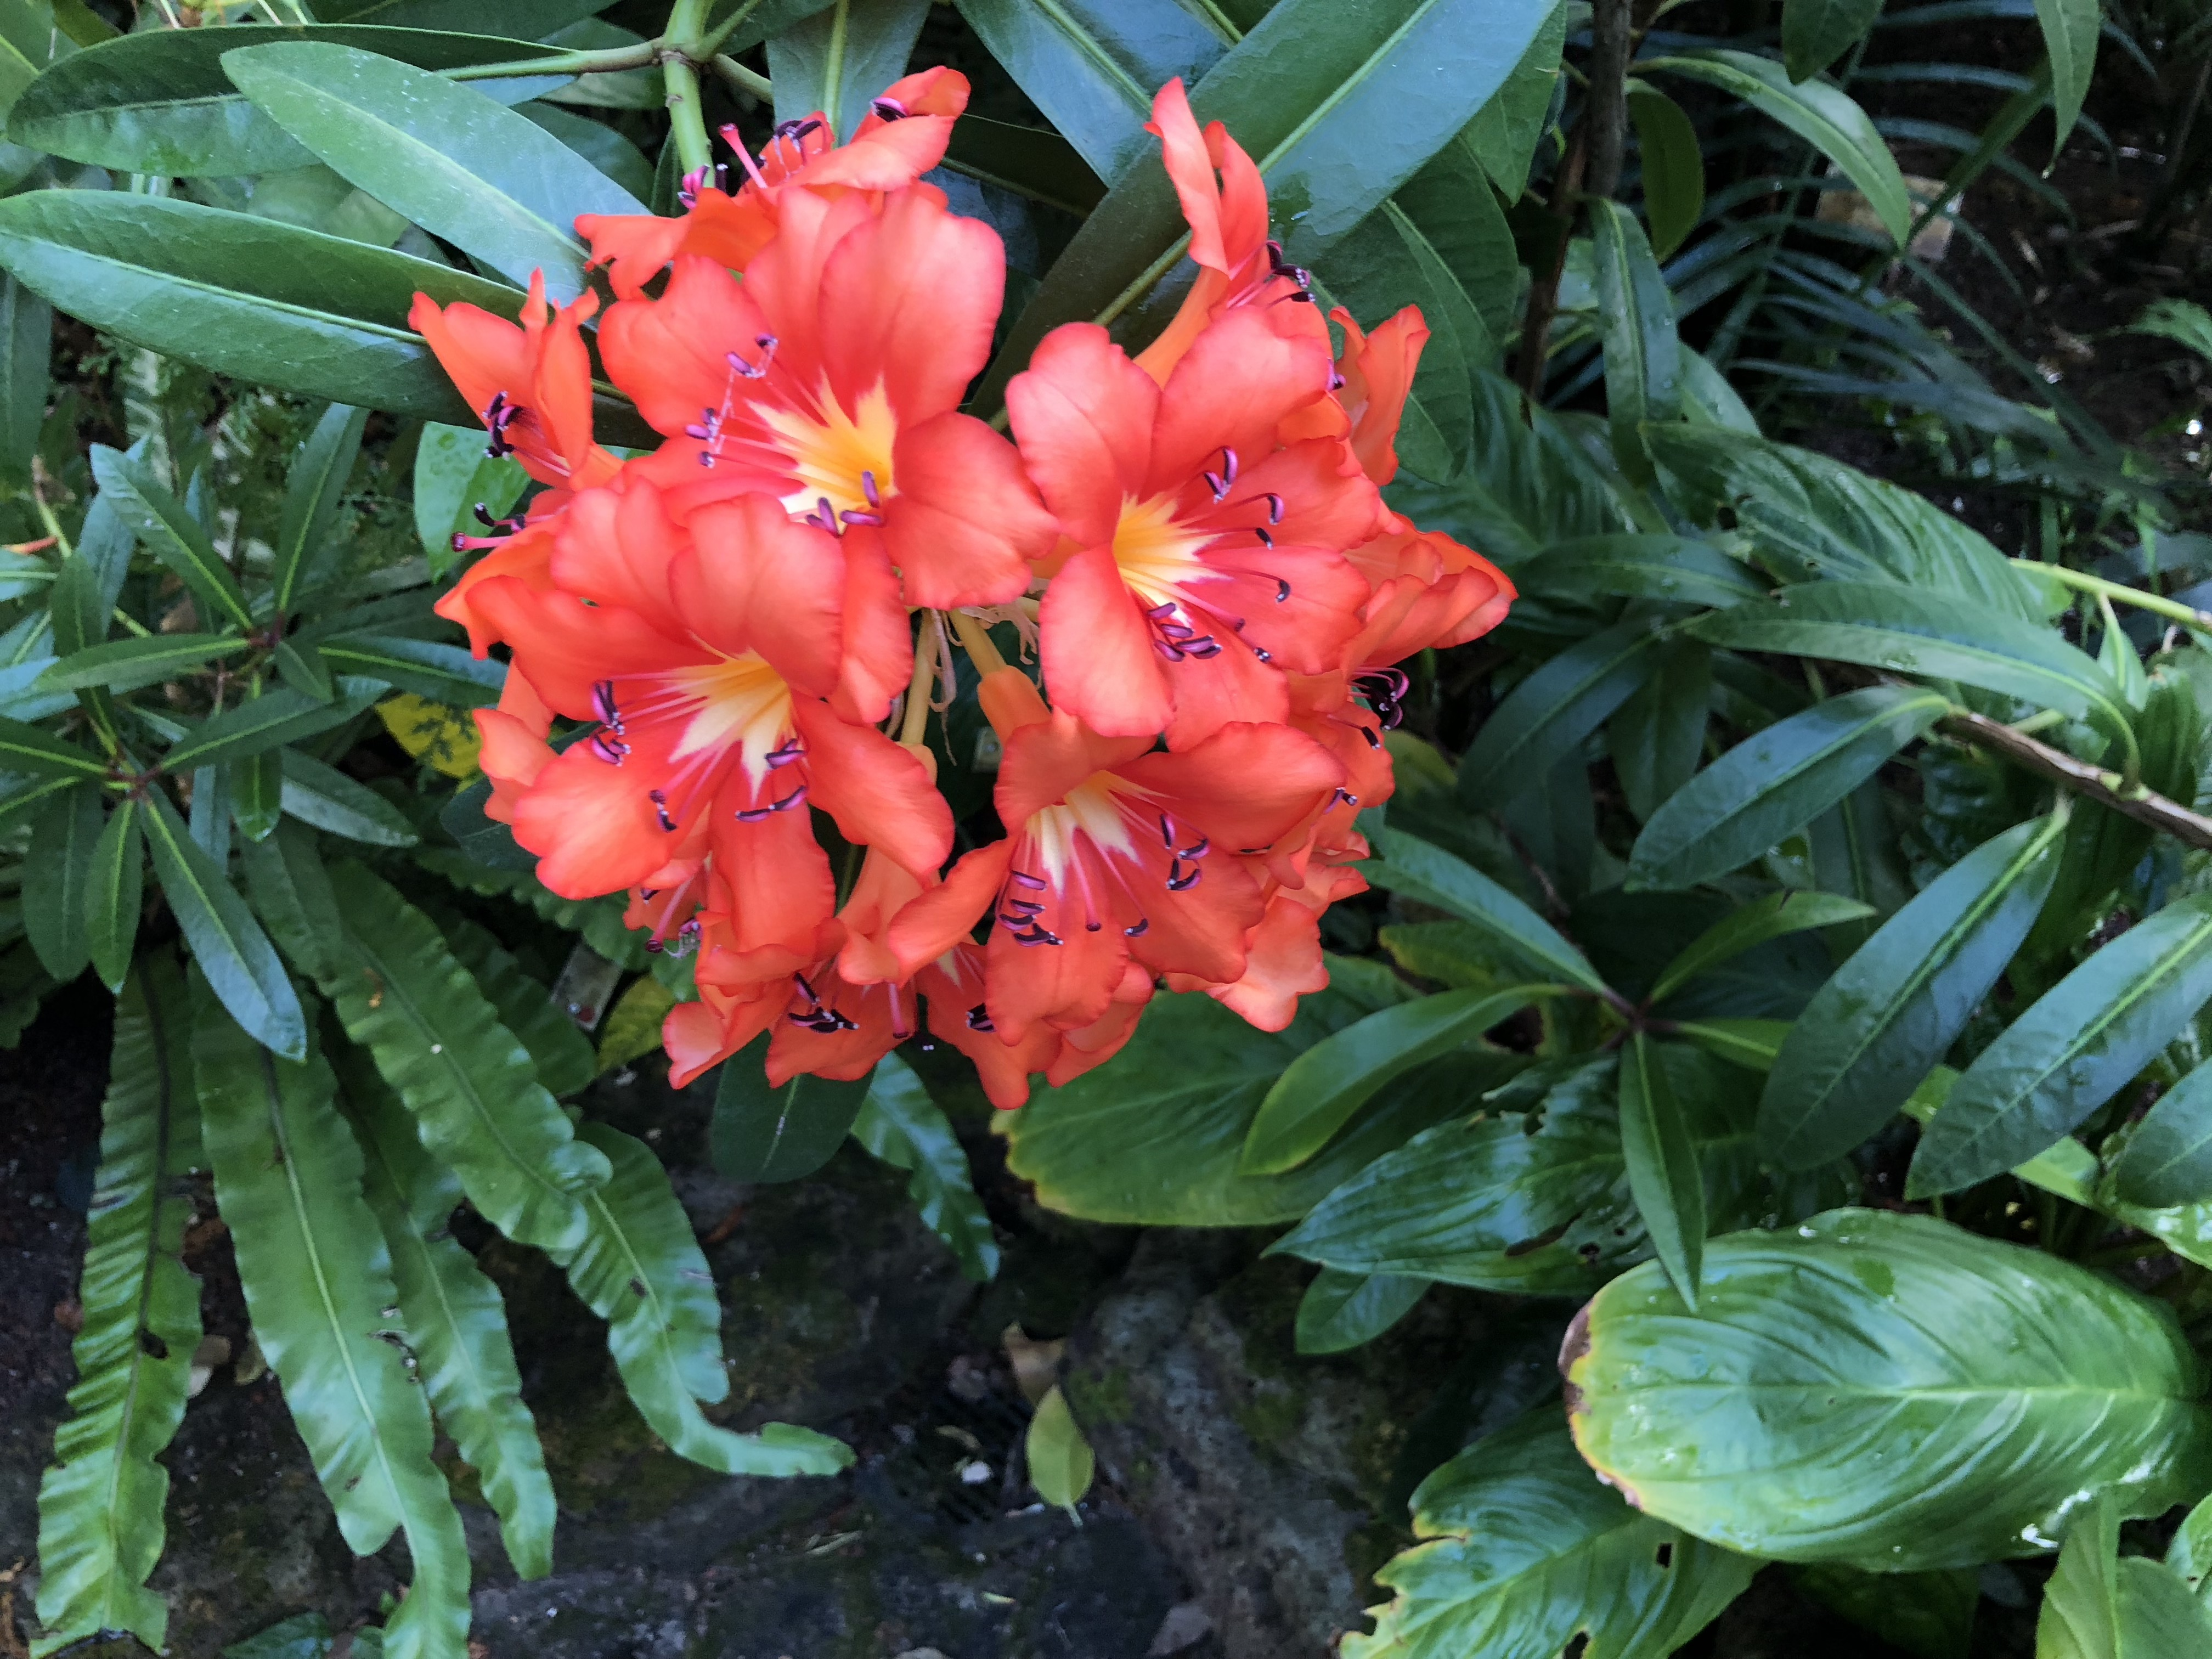
\includegraphics[width=\linewidth]{images/flower.jpg}
            \caption{Original Image}
        \end{subfigure}
        \hfill
        \begin{subfigure}[b]{0.45\linewidth}
            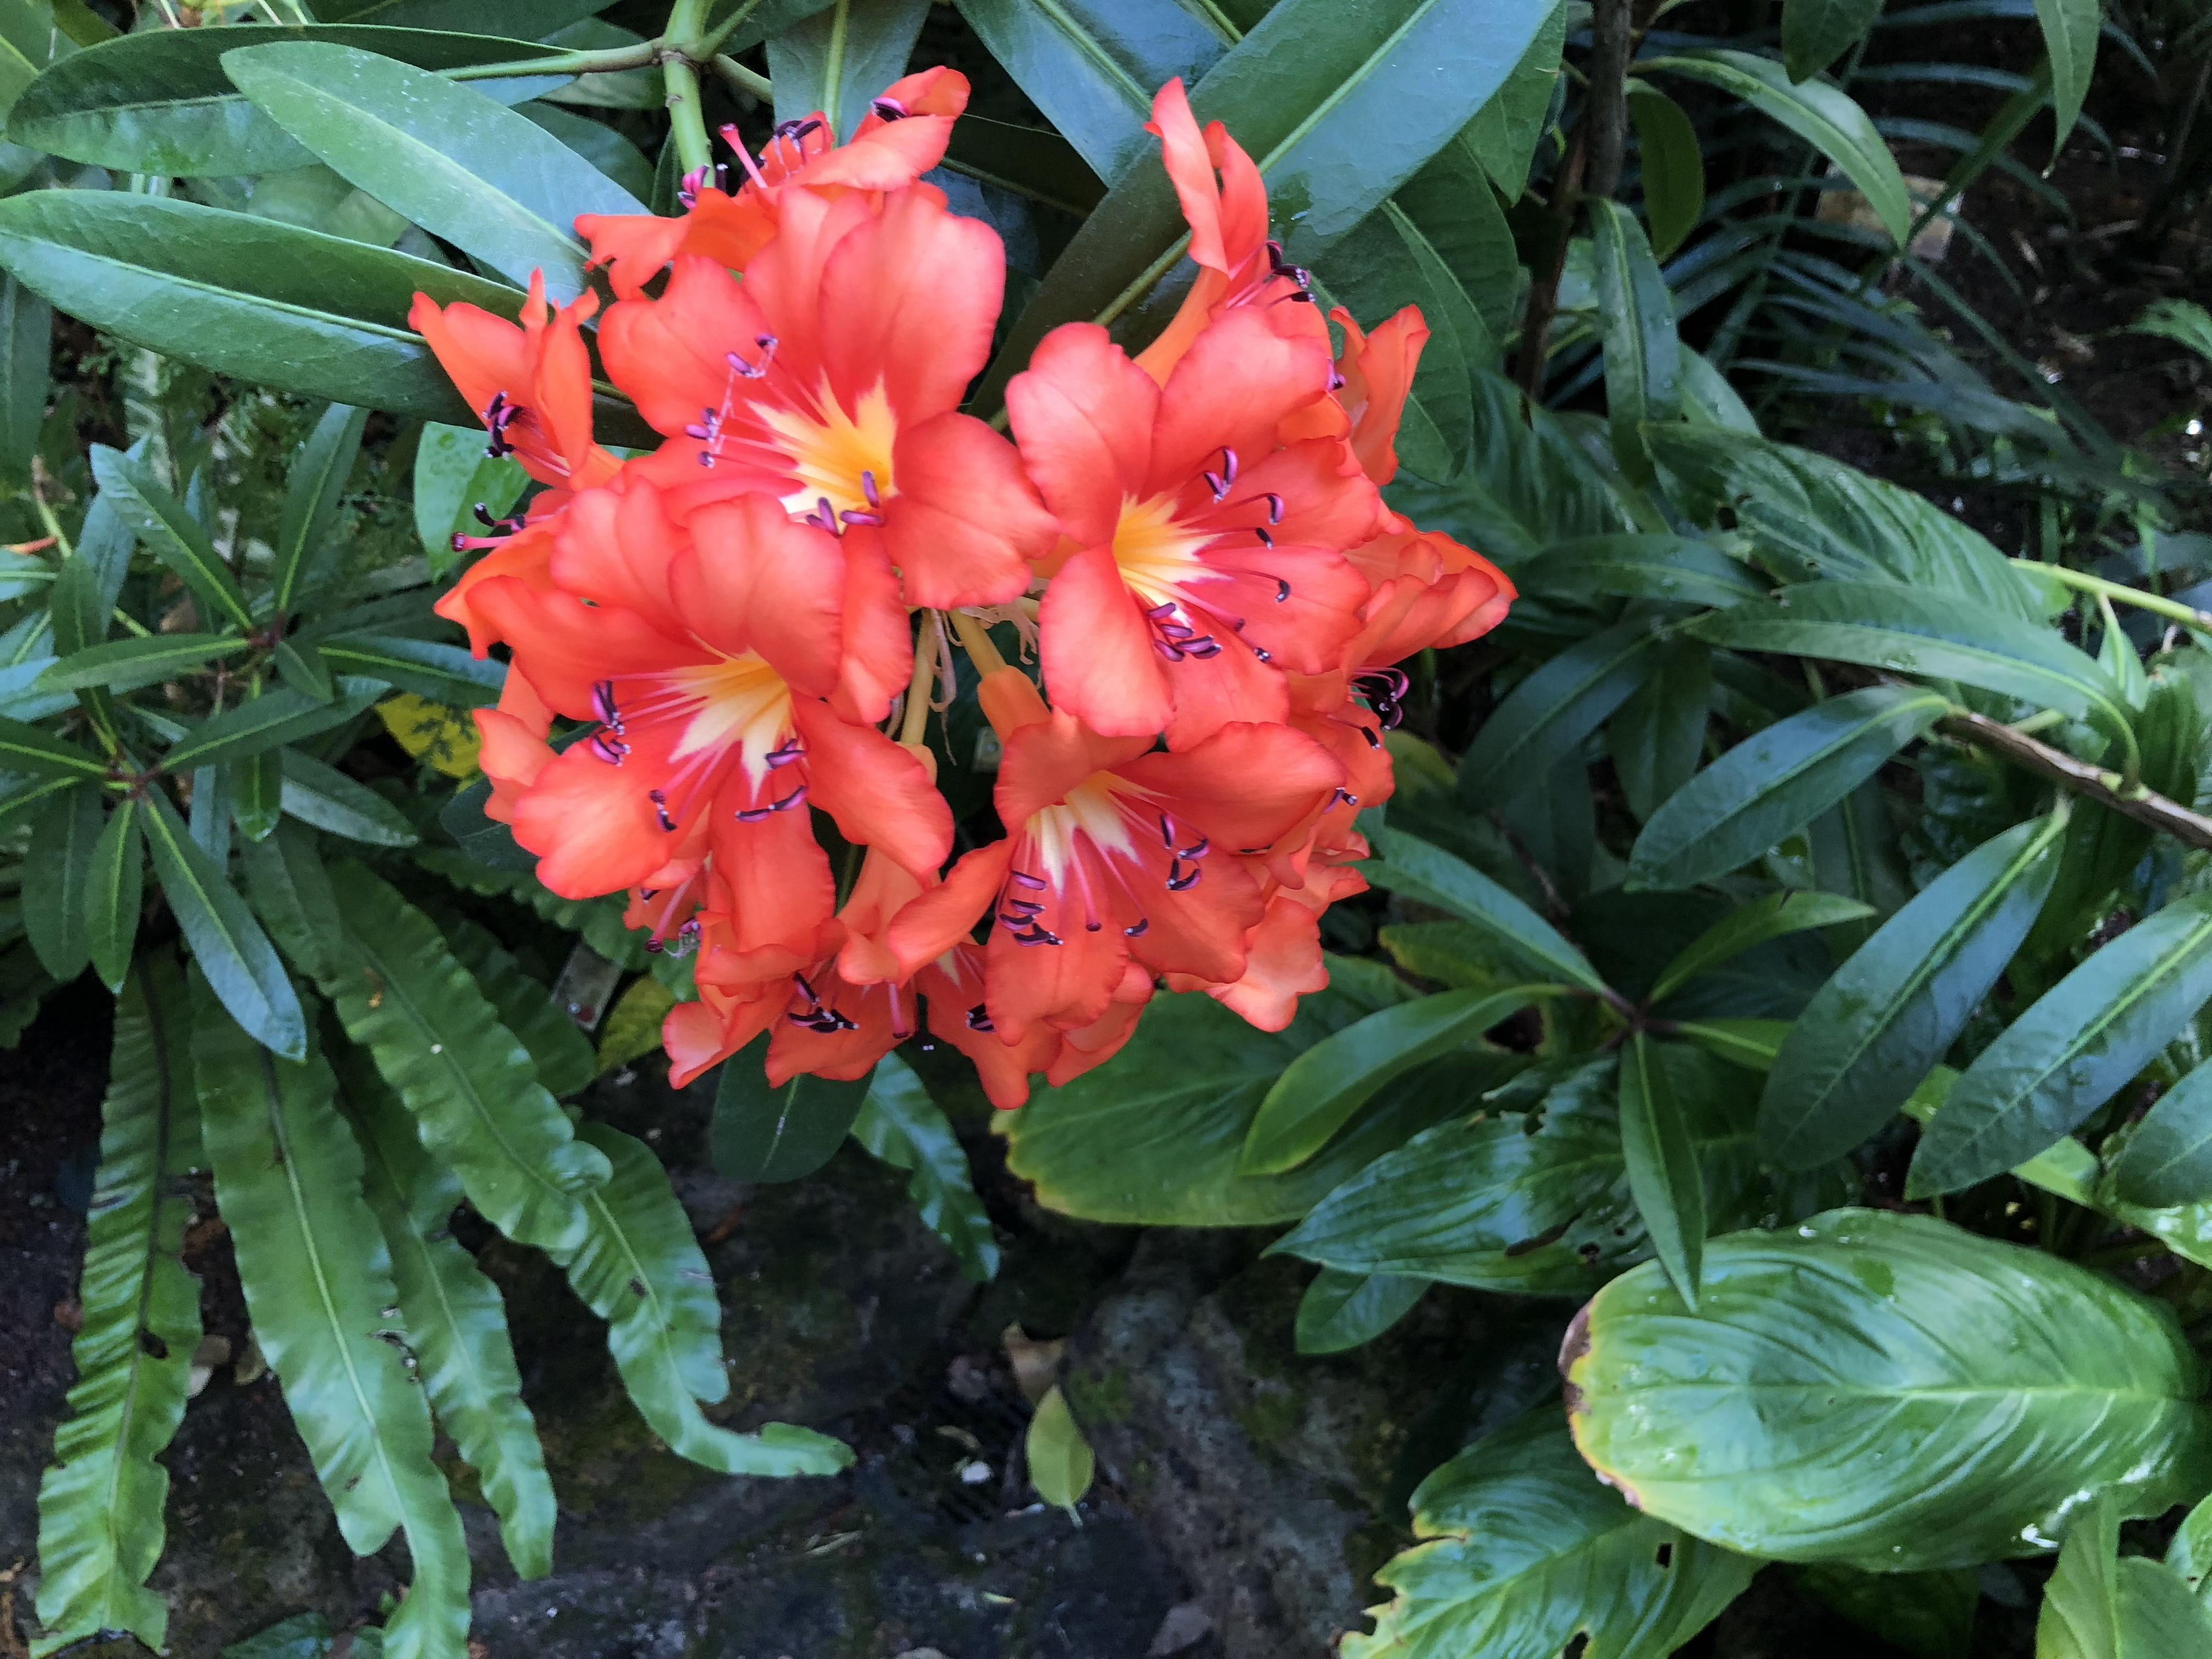
\includegraphics[width=\linewidth]{images/flower_recon.jpg}
            \caption{Reconstructed Image}
        \end{subfigure}

        \vspace{0.5cm}
        \begin{subfigure}[b]{0.45\linewidth}
            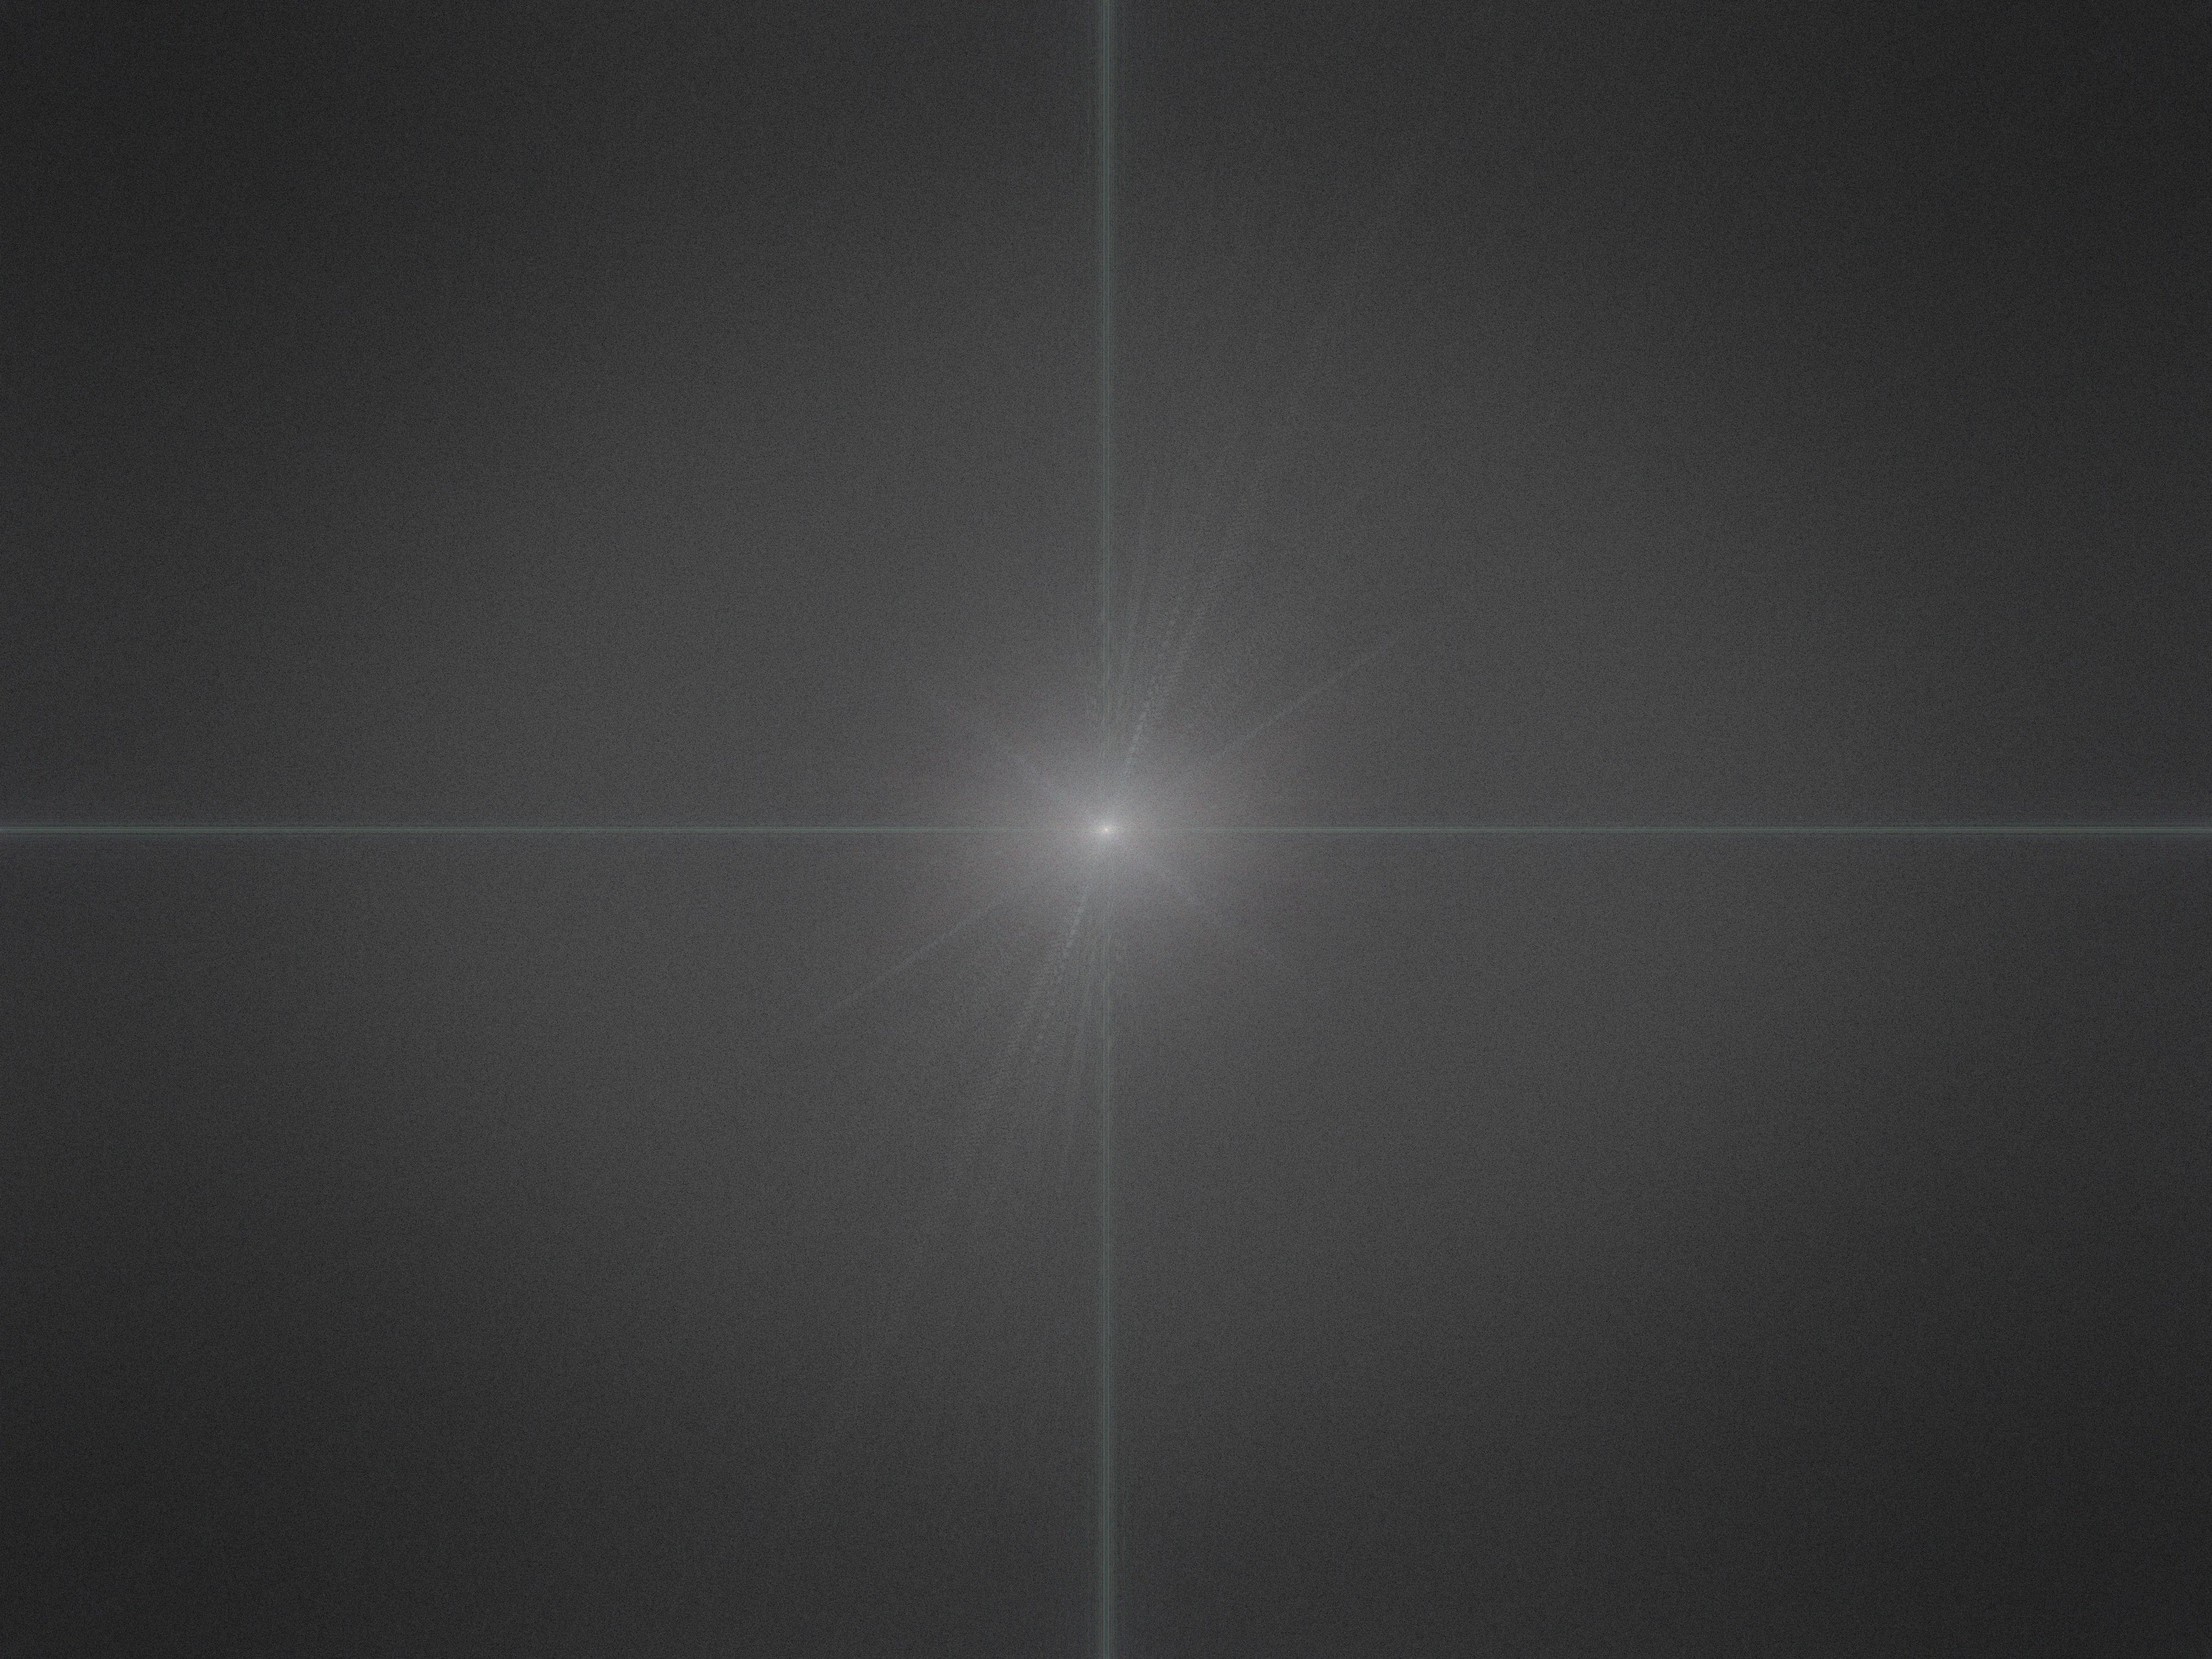
\includegraphics[width=\linewidth]{images/flower_magnitude.jpg}
            \caption{Magnitude}
        \end{subfigure}
        \hfill
        \begin{subfigure}[b]{0.45\linewidth}
            \includegraphics[width=\linewidth]{images/flower_phase.jpg}
            \caption{Phase}
        \end{subfigure}

        \vspace{0.5cm}
        \begin{subfigure}[b]{0.45\linewidth}
            \includegraphics[width=\linewidth]{images/flower_real.jpg}
            \caption{Real Part}
        \end{subfigure}
        \hfill
        \begin{subfigure}[b]{0.45\linewidth}
            \includegraphics[width=\linewidth]{images/flower_imag.jpg}
            \caption{Imaginary Part}
        \end{subfigure}

        \caption{Flower: Images generated during the DFT process}
        \label{fig:flower_1}
    \end{minipage}
\end{figure}

\begin{figure}[htbp]
    \centering 
    \begin{minipage}{0.8\textwidth} 
        \centering 
        
        \begin{subfigure}[b]{0.45\linewidth} 
            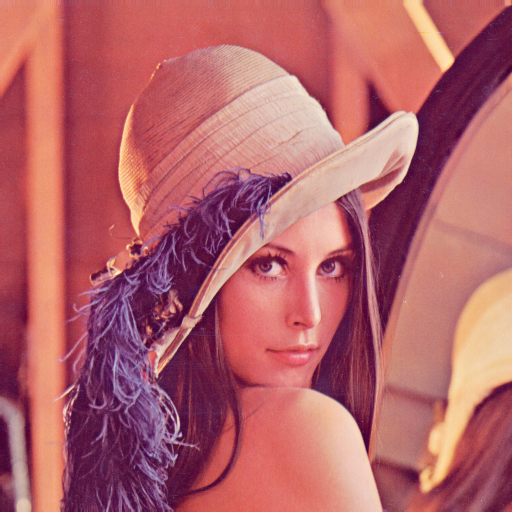
\includegraphics[width=\linewidth]{images/lena.png}
            \caption{Original Image}
        \end{subfigure}
        \hfill
        \begin{subfigure}[b]{0.45\linewidth}
            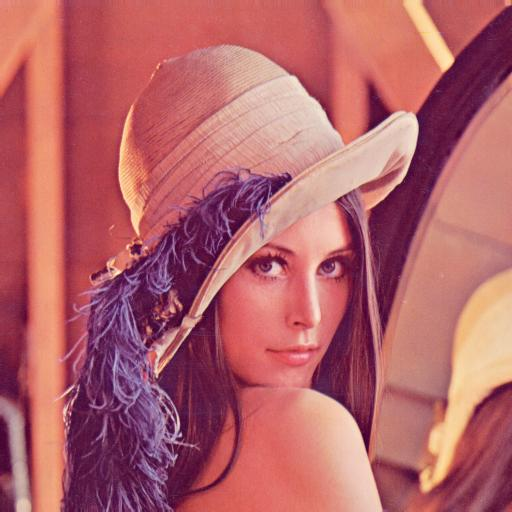
\includegraphics[width=\linewidth]{images/lena_recon.jpg}
            \caption{Reconstructed Image}
        \end{subfigure}

        \vspace{0.5cm}
        \begin{subfigure}[b]{0.45\linewidth}
            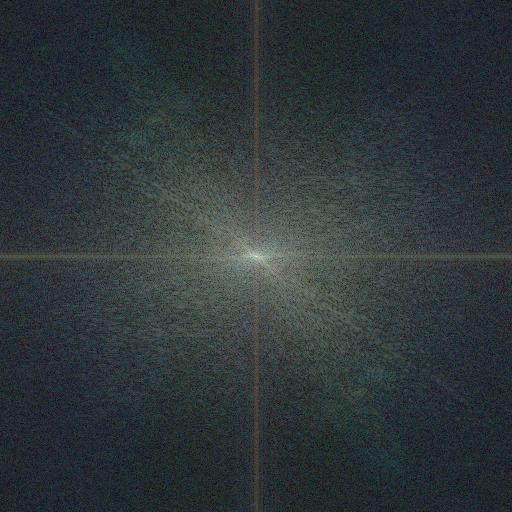
\includegraphics[width=\linewidth]{images/lena_magnitude.jpg}
            \caption{Magnitude}
        \end{subfigure}
        \hfill
        \begin{subfigure}[b]{0.45\linewidth}
            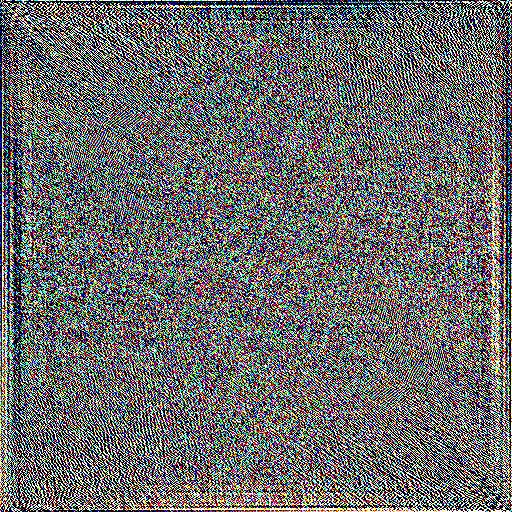
\includegraphics[width=\linewidth]{images/lena_phase.jpg}
            \caption{Phase}
        \end{subfigure}

        \vspace{0.5cm}
        \begin{subfigure}[b]{0.45\linewidth}
            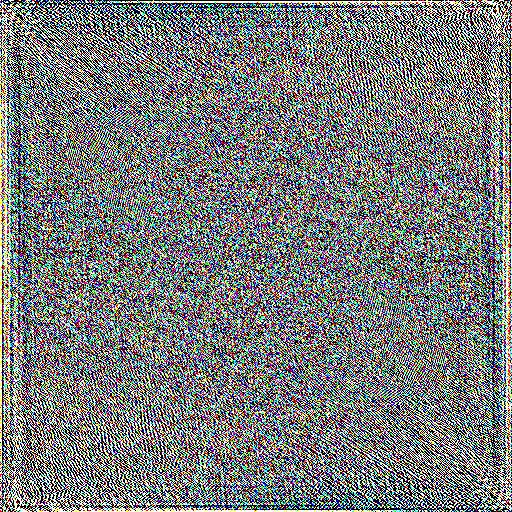
\includegraphics[width=\linewidth]{images/lena_real.jpg}
            \caption{Real Part}
        \end{subfigure}
        \hfill
        \begin{subfigure}[b]{0.45\linewidth}
            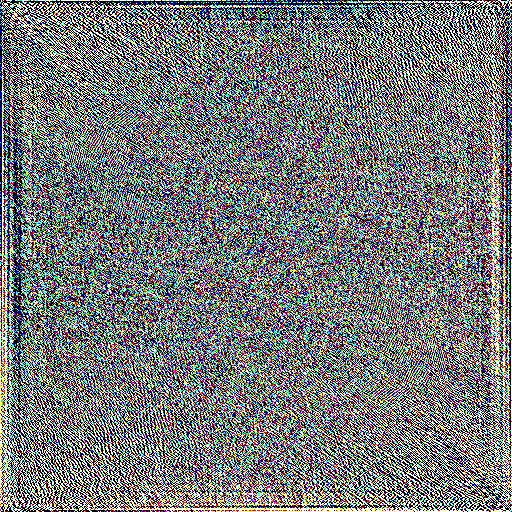
\includegraphics[width=\linewidth]{images/lena_imag.jpg}
            \caption{Imaginary Part}
        \end{subfigure}

        \caption{Lena: Images generated during the DFT process}
        \label{fig:lena_1}
    \end{minipage}
\end{figure}

\begin{figure}[htbp]
    \centering 
    \begin{minipage}{0.8\textwidth} 
        \centering 
        
        \begin{subfigure}[b]{0.45\linewidth} 
            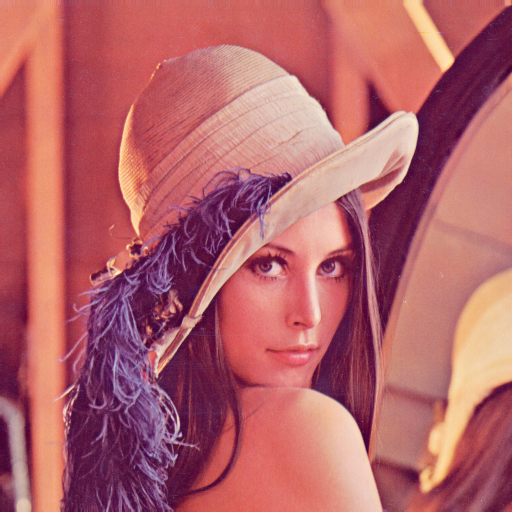
\includegraphics[width=\linewidth]{images/lena.png}
            \caption{Original Image}
        \end{subfigure}
        \hfill
        \begin{subfigure}[b]{0.45\linewidth}
            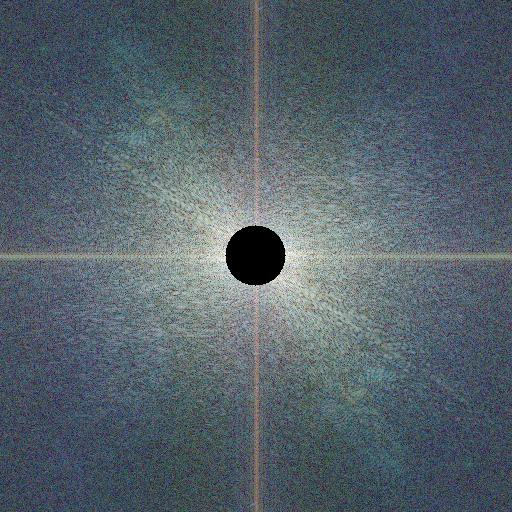
\includegraphics[width=\linewidth]{images/lena_mag_high_30.jpg}
            \caption{High-pass Filter}
        \end{subfigure}

        \vspace{0.5cm}
        \begin{subfigure}[b]{0.45\linewidth}
            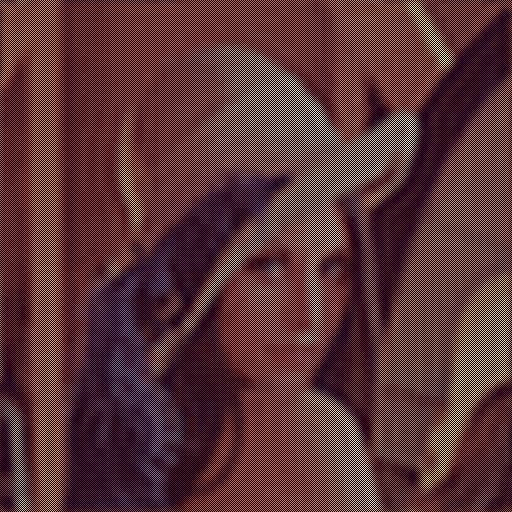
\includegraphics[width=\linewidth]{images/lena_low_30.jpg}
            \caption{Low-pass Image}
        \end{subfigure}
        \hfill
        \begin{subfigure}[b]{0.45\linewidth}
            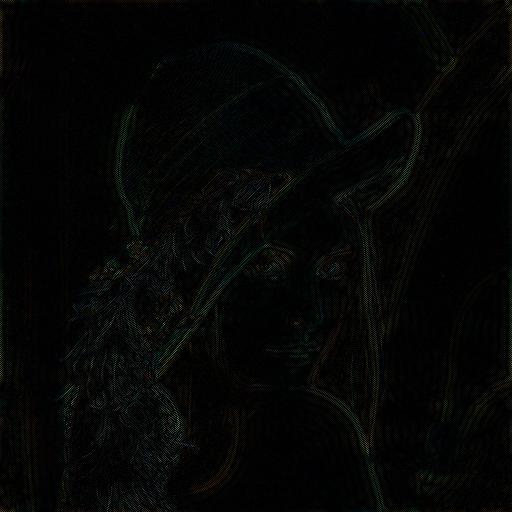
\includegraphics[width=\linewidth]{images/lena_high_30.jpg}
            \caption{High-pass Image}
        \end{subfigure}

        \caption{Lena: Comparison between the Original and Filtered Images with D0=30}
        \label{fig:lena_2}
    \end{minipage}
\end{figure}

\begin{figure}[htbp]
    \centering 
    \begin{minipage}{0.8\textwidth} 
        \centering 
        
        \begin{subfigure}[b]{0.45\linewidth} 
            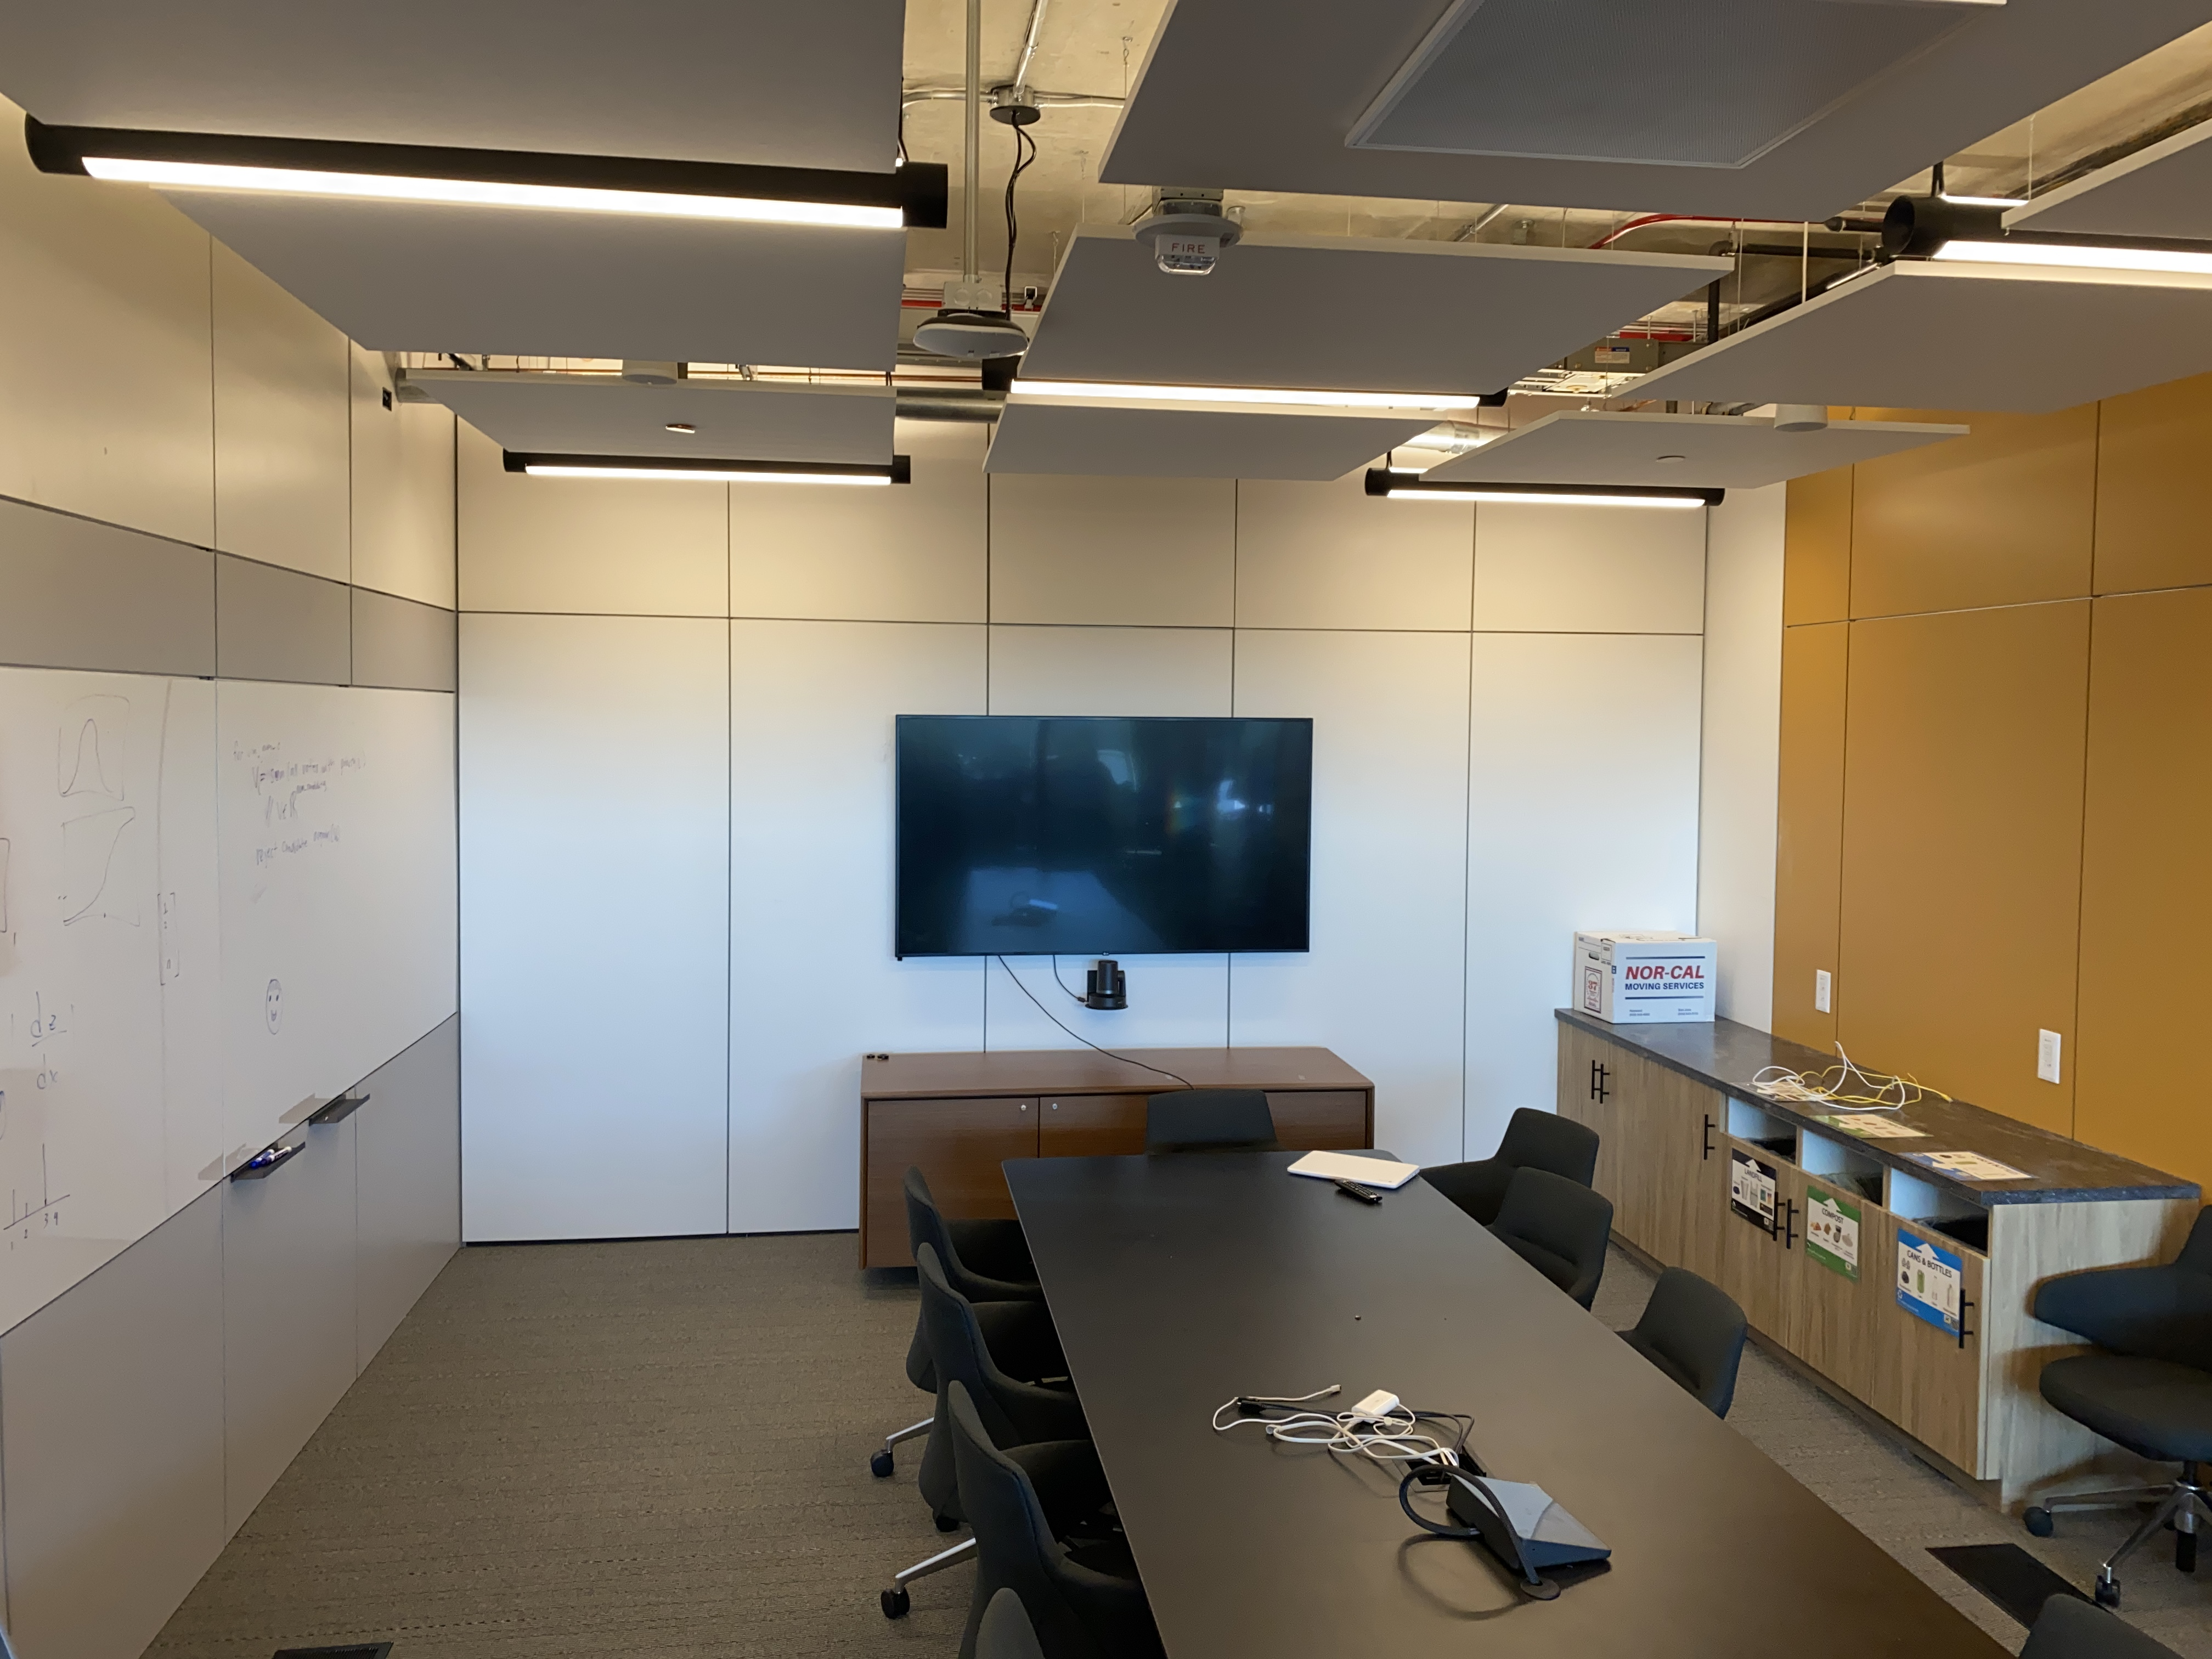
\includegraphics[width=\linewidth]{images/room.jpg}
            \caption{Original Image}
        \end{subfigure}
        \hfill
        \begin{subfigure}[b]{0.45\linewidth}
            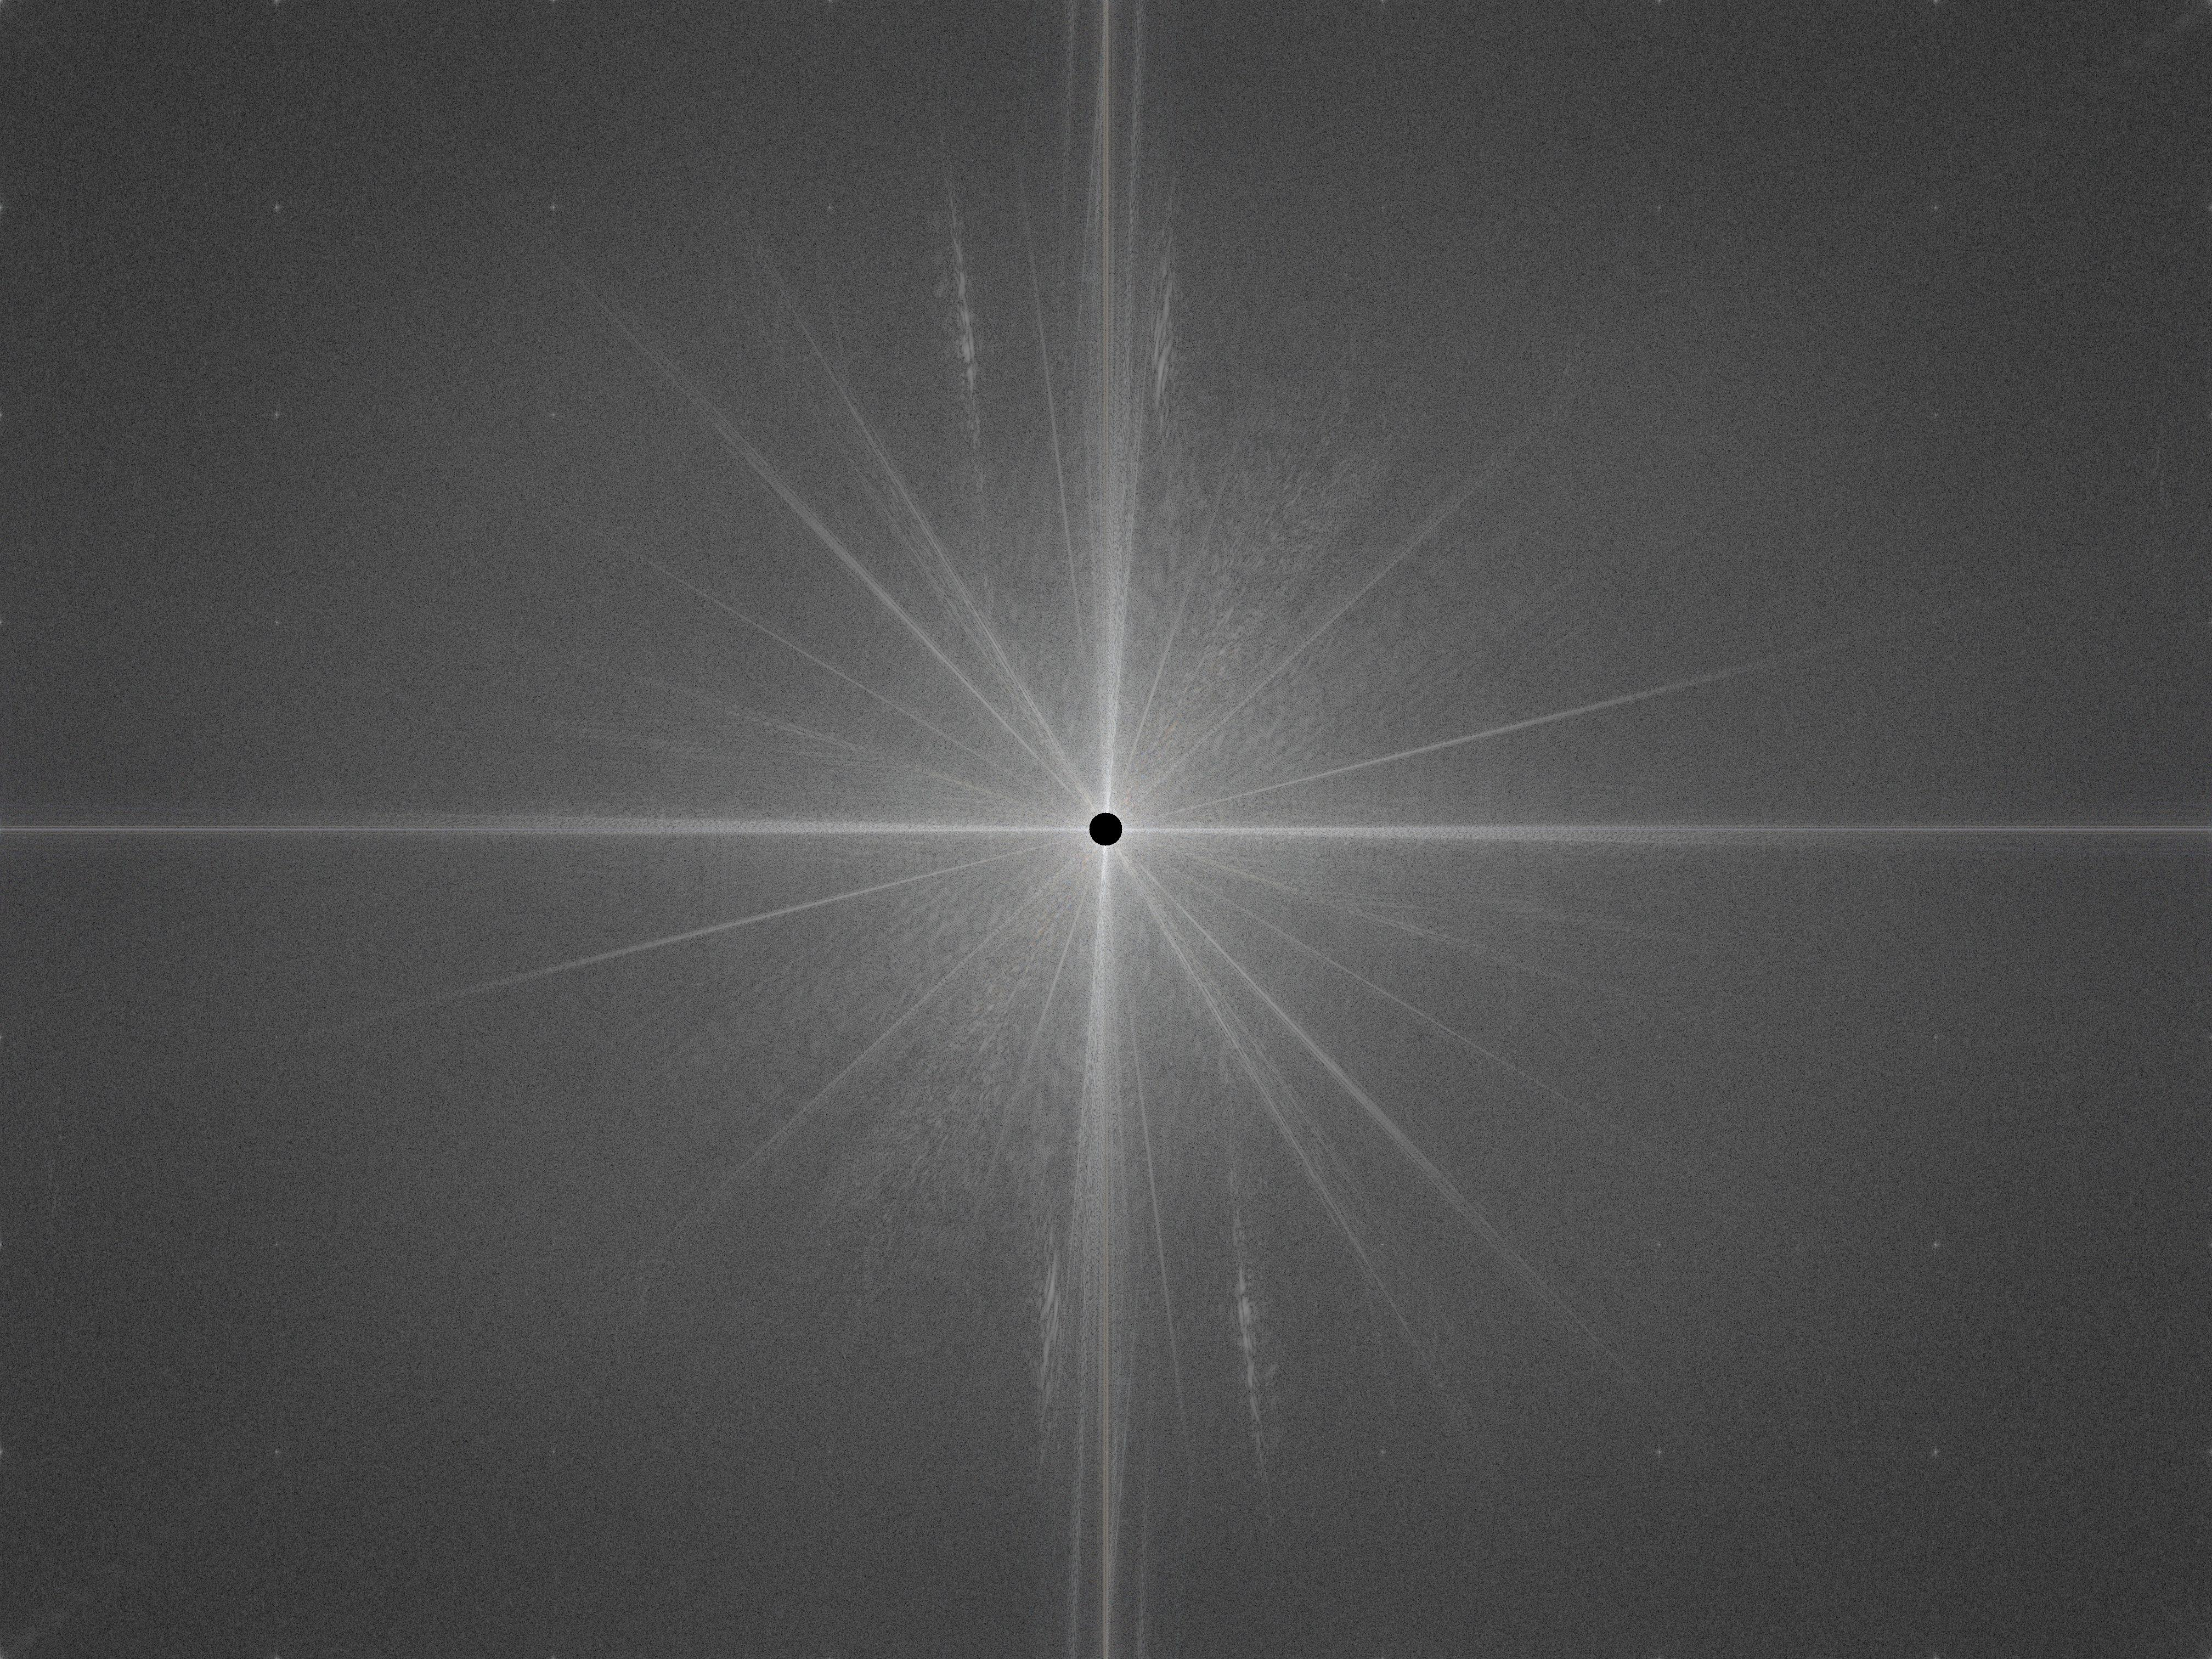
\includegraphics[width=\linewidth]{images/room_mag_high_30.jpg}
            \caption{High-pass Filter}
        \end{subfigure}

        \vspace{0.5cm}
        \begin{subfigure}[b]{0.45\linewidth}
            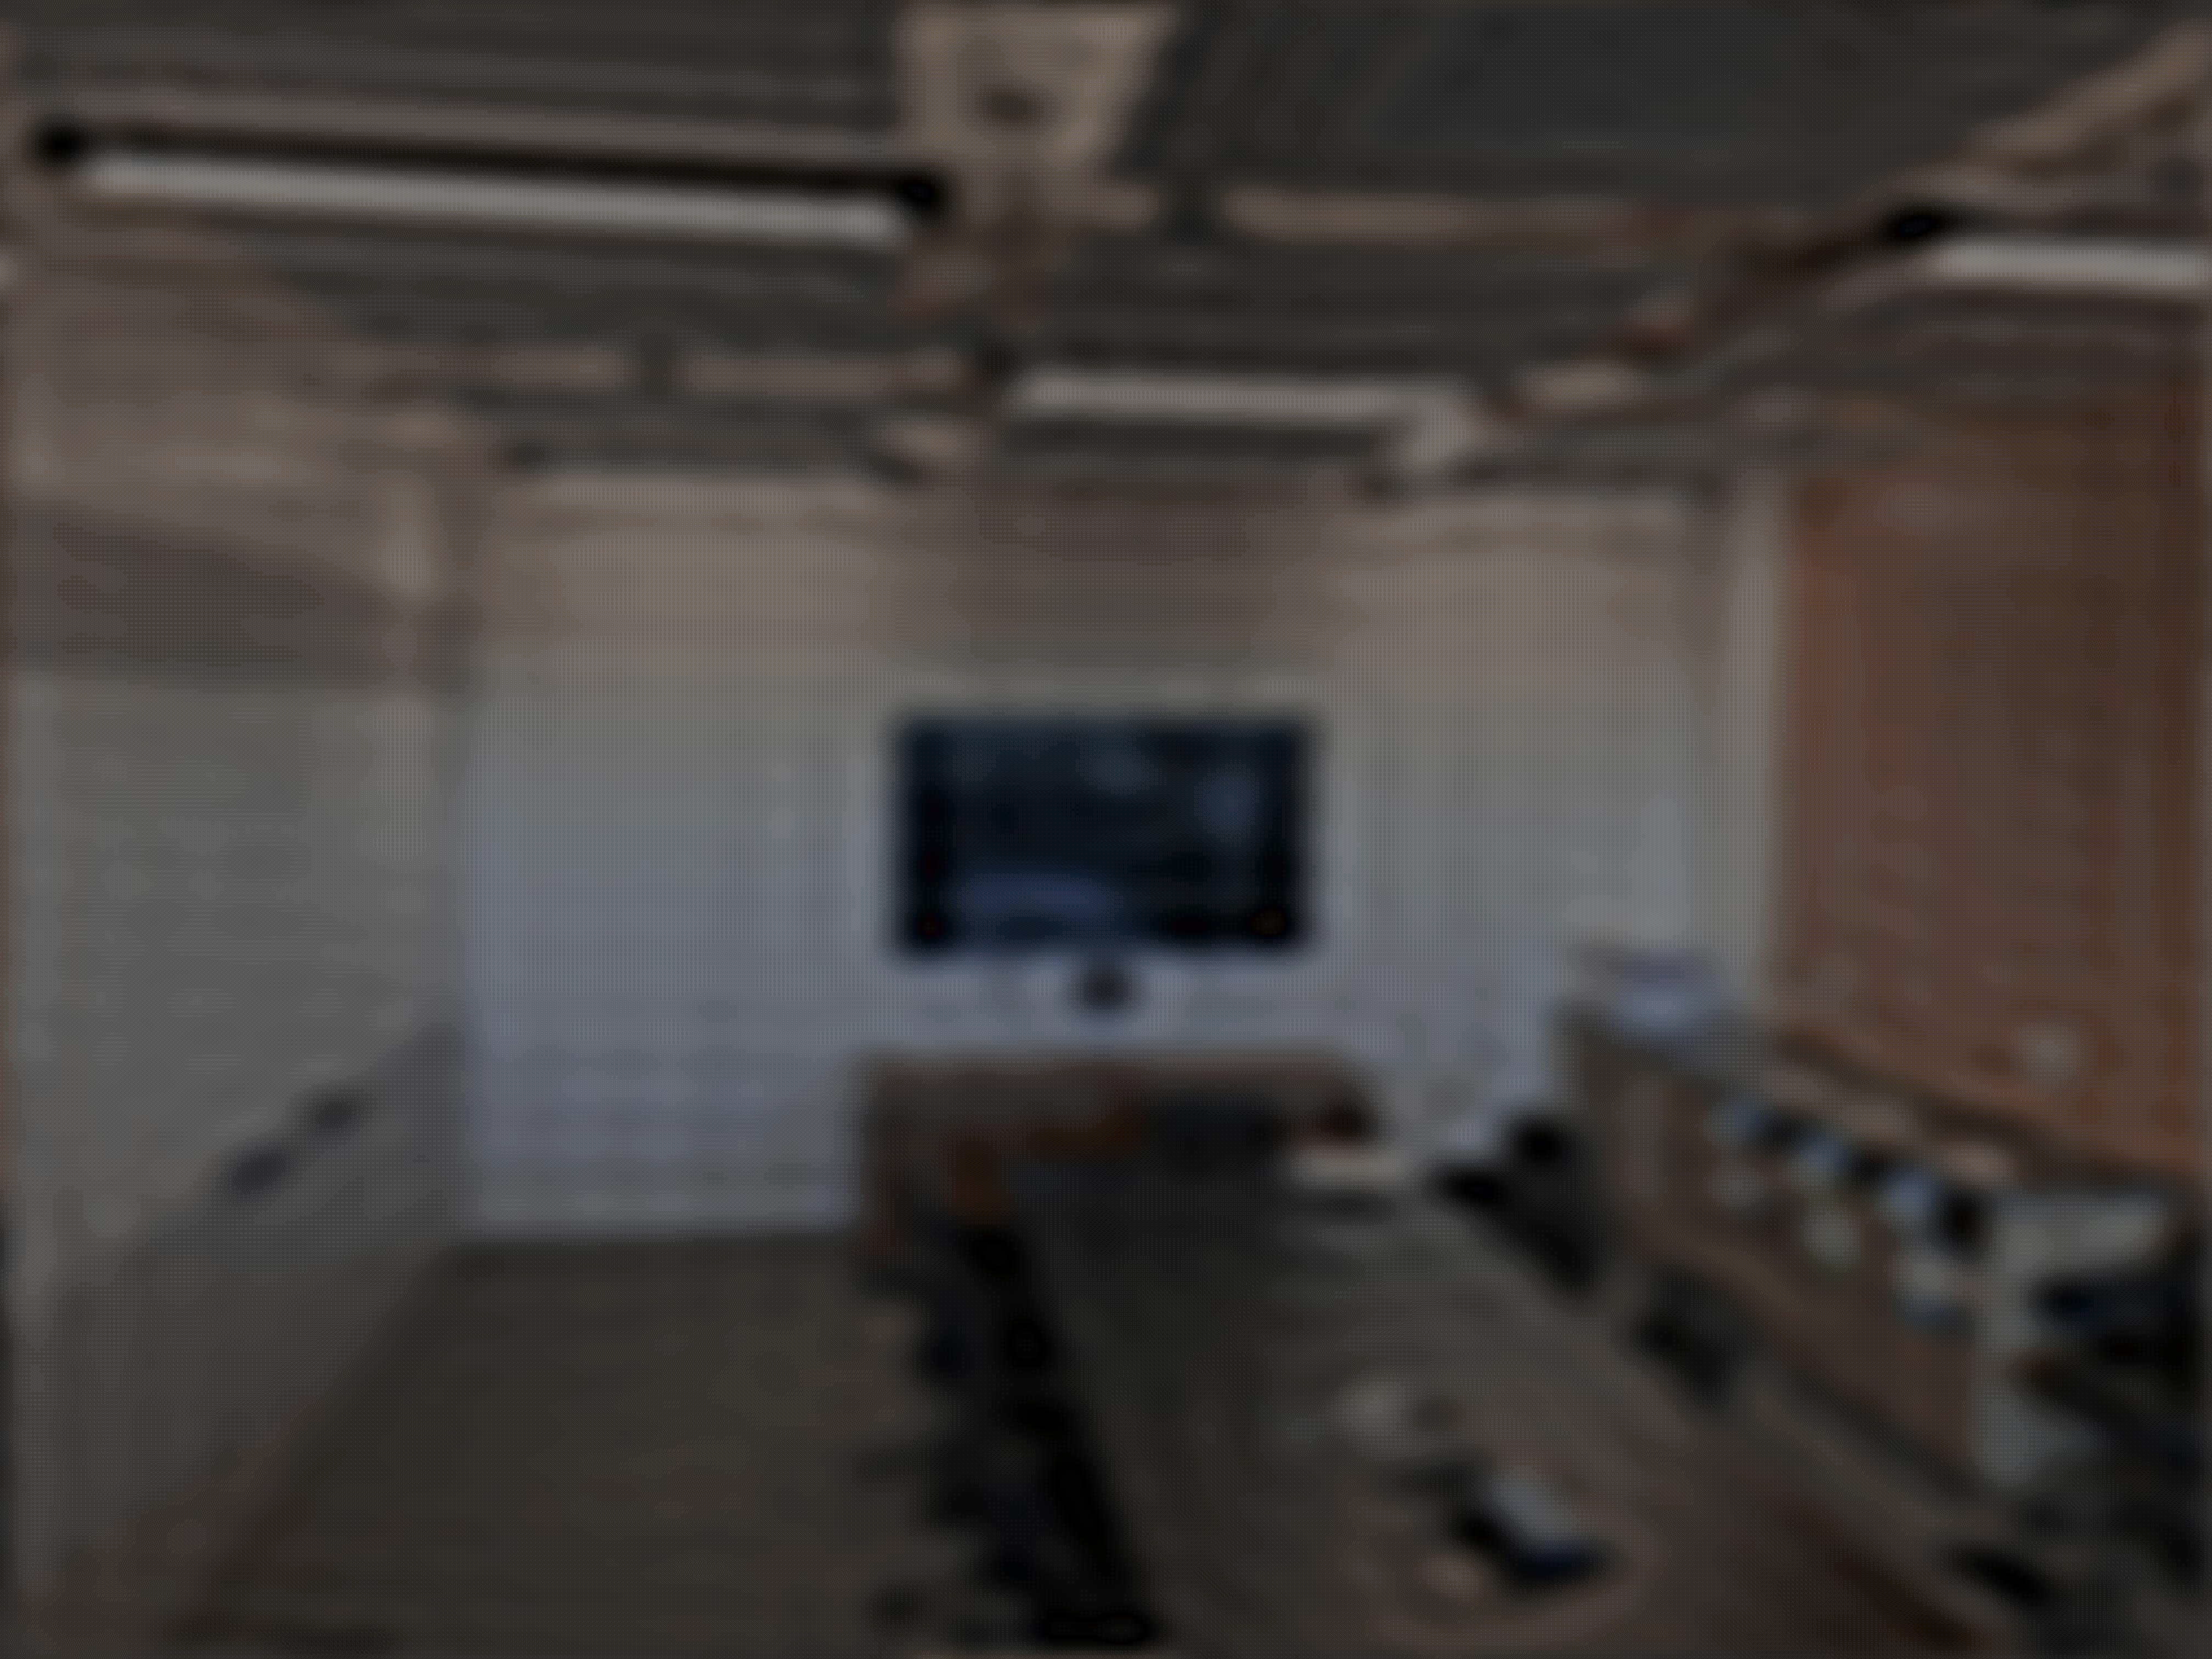
\includegraphics[width=\linewidth]{images/room_low_30.jpg}
            \caption{Low-pass Image}
        \end{subfigure}
        \hfill
        \begin{subfigure}[b]{0.45\linewidth}
            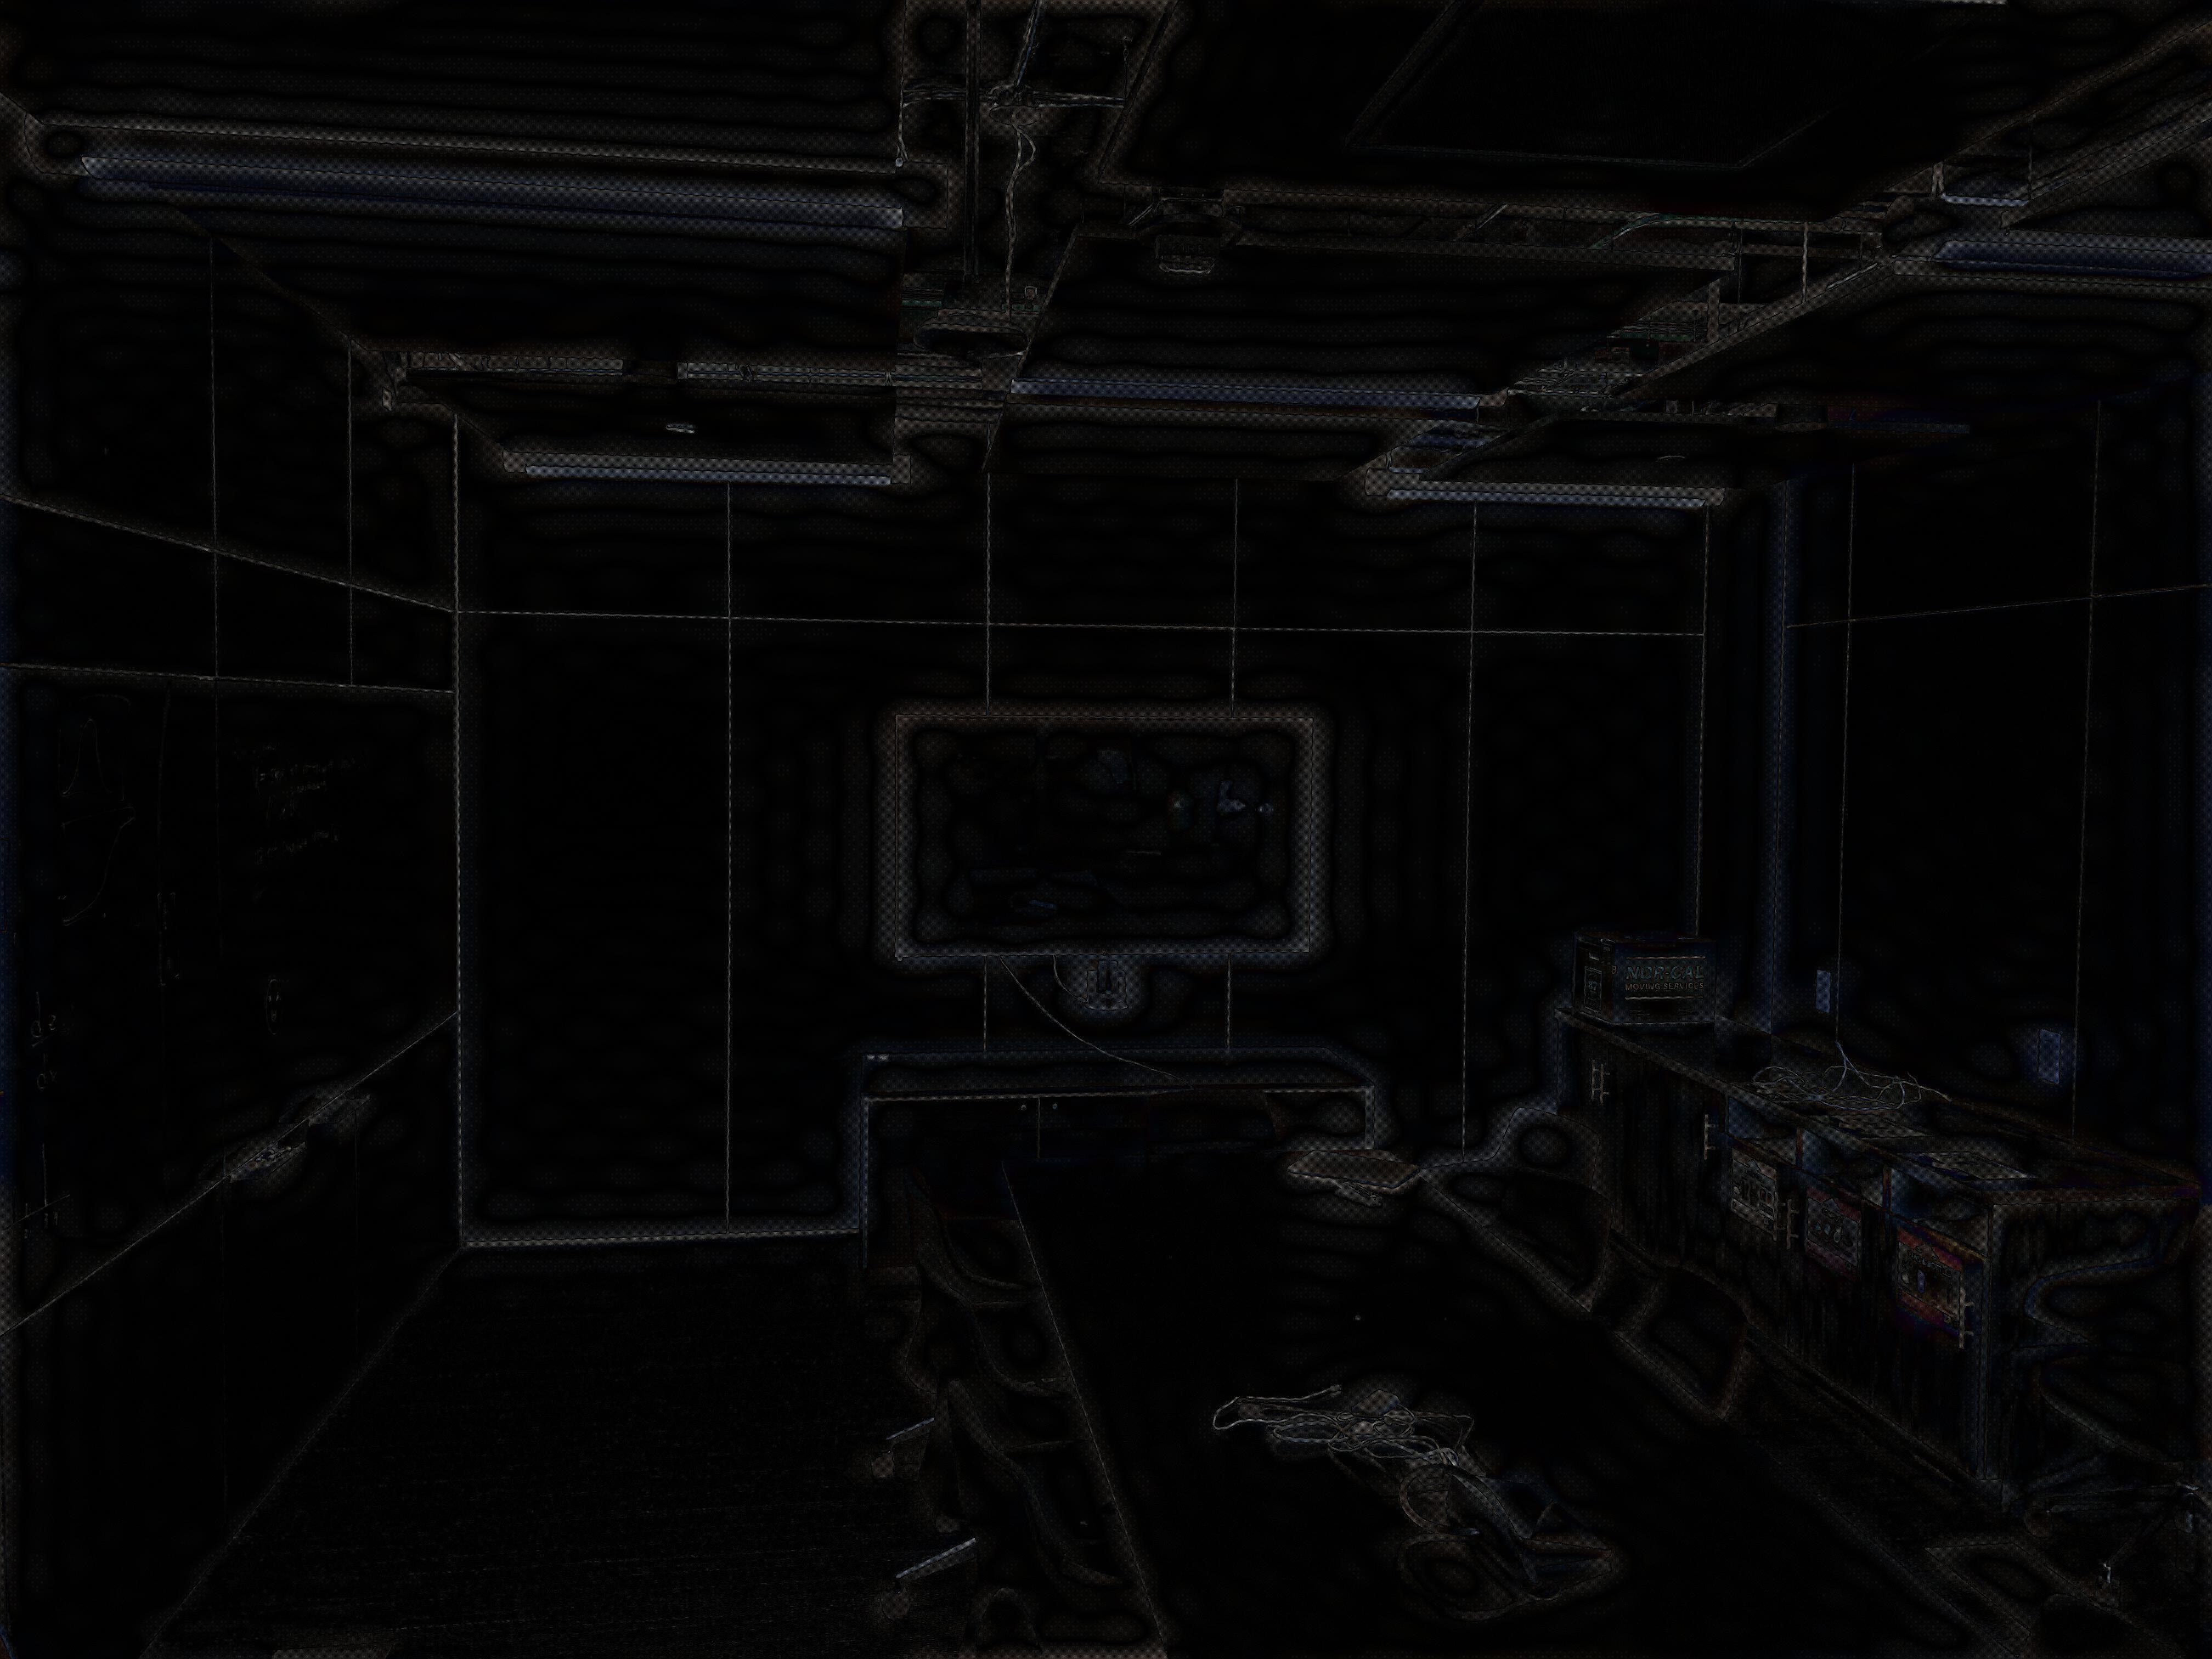
\includegraphics[width=\linewidth]{images/room_high_30.jpg}
            \caption{High-pass Image}
        \end{subfigure}

        \caption{Room: Comparison between the Original and Filtered Images with D0=30}
        \label{fig:room_2}
    \end{minipage}
\end{figure}





% =================================================

% \newpage

% \vfill

% \bibliographystyle{ieeetr}
% \bibliography{references}

\end{document}